\section{El grupo fundamental}
\begin{ejercicio}
    Prueba que en un espacio topológico simplemente conexo $X$, dos arcos cualesquiera $\alpha,\beta\in \Omega(X,x,y)$ son homotópicos por arcos.\\

    \noindent
    Sean $\alpha,\beta\in \Omega(X,x,y)$, tenemos que $\alpha\ast\tilde{\beta}$ es un lazo basado en $x$, y por ser $X$ simplemente conexo tenemos que $\left[\alpha\ast\tilde{\beta}\right] = [\varepsilon_x]$, de donde:
    \begin{equation*}
        [\alpha]\ast\left[\tilde{\beta}\right] = \left[\alpha\ast\tilde{\beta}\right] = [\varepsilon_x] \Longrightarrow [\alpha] = [\beta]
    \end{equation*}
\end{ejercicio}

\begin{ejercicio}
    Sean $X$ un subconjunto de $\mathbb{R}^n$ y $f:X\to Y$ una aplicación. Demuestra que si $f$ se puede extender a una aplicación continua $F:\mathbb{R}^n\to Y$, entonces $f_\ast$ es el homomorfismo trivial, es decir, el homomorfismo que lleva todo elemento en el neutro.\\

    \noindent
    Como $F$ es una extensión de $f$, tenemos que $F\circ i = f$, es decir:
    \begin{figure}[H]
        \centering
        \shorthandoff{""}
        \begin{tikzcd}
            {X} \arrow[r, "i", hook] \arrow[rr, "f", bend right] & {\mathbb{R}^n} \arrow[r, "F"] & {Y}
        \end{tikzcd}
        \shorthandon{""}
    \end{figure}
    \noindent
    Y como cada una de ellas es continua ($f$ es continua por ser $f=F\big|_X$), podemos inducir el diagrama a grupos fundamentales, obteniendo para cada $x_0\in X$:
    \begin{figure}[H]
        \centering
        \shorthandoff{""}
        \begin{tikzcd}
            {\pi_1(X,x_0)} \arrow[r, "i_\ast", hook] \arrow[rr, "f_\ast", bend right=49] & {\pi_1(\mathbb{R}^n,x_0)} \arrow[r, "F_\ast"] & {\pi_1(Y,f(x_0))}
        \end{tikzcd}
        \shorthandon{""}
    \end{figure}
    de donde:
    \begin{equation*}
        f_\ast([\alpha]_X) = F_\ast(i_\ast([\alpha]_{X})) = F_\ast({[\alpha]}_{\bb{R}^n}) \AstIg F_\ast([\varepsilon_{x_0}]_{\mathbb{R}^n}) = [\varepsilon_{f(x_0)}]_Y \qquad \forall [\alpha]_X \in \pi_1(X,x_0)
    \end{equation*}
    donde en $(\ast)$ hemos usado que $\mathbb{R}^n$ es simplemente conexo.
\end{ejercicio}

\begin{ejercicio}
    Se dice que un grupo $G$ con operación $\cdot $ es un grupo topológico si $G$ tiene una topología de forma que las aplicaciones producto e inversión
    \Func{}{G\times G}{G}{(x,y)}{x\cdot y} \Func{}{G}{G}{x}{x^{-1}}
    son continuas. Sea e el elemento neutro en $G$:
    \begin{enumerate}[label=\alph*)]
        \item Dados $\alpha,\beta\in \Omega(G,e)$, se define $\alpha\cdot \beta:[0,1]\to G$ como $(\alpha\cdot \beta)(t) = \alpha(t)\cdot \beta(t)$. Demuestra que $\alpha\cdot \beta\in \Omega(G,e)$.

            Hemos de probar que $\alpha\cdot \beta$ es un lazo basado en $e$. Para ello:
            \begin{itemize}
                \item $\alpha\cdot \beta$ es continua, puesto que si consideramos:
                    \Func{\Phi}{G\times G}{G}{(x,y)}{x\cdot y}            
                    \Func{\Psi}{[0,1]}{G\times G}{t}{(\alpha(t), \beta(t))}
                    Tenemos que $\alpha\cdot \beta = \Phi \circ \Psi$:
                    \begin{equation*}
                        (\alpha\cdot \beta)(t) = \alpha(t)\cdot \beta(t) = \Phi(\alpha(t),\beta(t)) = \Phi(\Psi(t)) \qquad \forall t\in [0,1]
                    \end{equation*}
                    con $\Phi$ continua por hipótesis y $\Psi$ continua por ser $\Psi=(\alpha,\beta)$, con sus dos componentes funciones continuas, por ser arcos.
                \item Observemos que:
                    \begin{align*}
                        (\alpha\cdot \beta)(0) &= \alpha(0) \cdot \beta(0) = e\cdot e = e \\
                        (\alpha\cdot \beta)(1) &= \alpha(1) \cdot \beta(1) = e\cdot e = e \\
                    \end{align*}
            \end{itemize}
            Con lo que $\alpha\cdot \beta\in \Omega(G,e)$.
        \item Comprueba que $(\alpha\ast \varepsilon_e)\cdot (\varepsilon_e\ast \beta)=\alpha\ast \beta$ para cualesquiera $\alpha,\beta\in \Omega(G,e)$.

            Sean $\alpha,\beta\in \Omega(G,e)$, tenemos que:
            \begin{align*}
                ((\alpha\ast \varepsilon_e)&\cdot (\varepsilon_e\ast \beta))(t) = (\alpha\ast \varepsilon_e)(t)\cdot (\varepsilon_e\ast \beta)(t)  \\ &= \left\{\begin{array}{ll}
                    \alpha(2t)\cdot \varepsilon_e(2t) & \text{si\ } 0\leq t \leq \nicefrac{1}{2} \\
                    \varepsilon_e(2t-1)\cdot \beta(2t-1) & \text{si\ } \nicefrac{1}{2}\leq t \leq 1
                \end{array}\right.  \\
               &= \left\{\begin{array}{ll}
                   \alpha(2t)\cdot e & \text{si\ } 0\leq t \leq \nicefrac{1}{2} \\
                   e\cdot \beta(2t-1) & \text{si\ } \nicefrac{1}{2}\leq t\leq 1
           \end{array}\right\} = \left\{\begin{array}{ll}
               \alpha(2t) & \text{si\ } 0\leq t \leq \nicefrac{1}{2} \\
               \beta(2t-1) & \text{si\ } \nicefrac{1}{2}\leq t \leq 1
           \end{array}\right.\\ &= (\alpha\ast \beta)(t) \qquad \forall t\in [0,1]
            \end{align*}

        \item Sean $[\alpha],[\beta]\in \pi_1(G,e)$. Prueba que la operación $[\alpha]\cdot [\beta]=[\alpha\cdot \beta]$ está bien definida.

            Sean $\alpha,\alpha',\gamma,\gamma'\in \Omega(G,e)$ de forma que:
            \begin{equation}\label{eq:igualdades_ej3rel2}
                [\alpha] = [\alpha'], \qquad [\gamma] = [\gamma']
            \end{equation}
            hemos de probar que $[\alpha\cdot \gamma] = [\alpha'\cdot \gamma']$. De las igualdades~(\ref{eq:igualdades_ej3rel2}) sabemos que existen $H_1,H_2:[0,1]\times [0,1]\to G$ aplicaciones continuas con:
            \begin{gather*}
                H_1(s,0) = \alpha(s),\qquad  H_1(s,1) = \alpha'(s),\qquad  H_1(0,t) = e = H_1(1,t) \\
                H_2(s,0) = \gamma(s),\qquad  H_2(s,1) = \gamma'(s),\qquad  H_2(0,t) = e = H_2(1,t) 
            \end{gather*}
            Si definimos $H:[0,1]\times[0,1]\to G$ dada por:
            \begin{equation*}
                H(s,t) = H_1(s,t)\cdot H_2(s,t) \qquad \forall (s,t)\in [0,1]\times[0,1]
            \end{equation*}
            tenemos que $H$ es continua, ya que podemos verla como $H = \Phi\circ (H_1,H_2)$, al igual que inicmos en el apartado a), así como que:
            \begin{gather*}
                H(s,0) = H_1(s,0)\cdot H_2(s,0) = \alpha(s)\cdot \gamma(s) = (\alpha\cdot \gamma)(s) \\
                H(s,1) = H_1(s,1)\cdot H_2(s,1) = \alpha'(s)\cdot \gamma'(s) = (\alpha'\cdot \gamma')(s) \\
                H(0,t) = H_1(0,t)\cdot H_2(0,t) = e\cdot e = e = e\cdot e = H_1(1,t)\cdot H_2(1,t) = H(1,t)
            \end{gather*}
            Con lo que $H$ es una homotopía, lo que nos dice que $[\alpha\cdot \gamma] = [\alpha'\cdot \gamma']$, luego la operación está bien definida.
        \item Muestra que $[\alpha]\cdot [\beta]=[\alpha]\ast[\beta]$, para cada $[\alpha],[\beta]\in \pi_1(G,e)$.
            \begin{equation*}
                [\alpha]\cdot [\beta] = [\alpha\ast \varepsilon_e] \cdot [\varepsilon_e\ast \beta] = [(\alpha\ast\varepsilon_e)\cdot (\varepsilon_e\ast\beta)] \stackrel{b)}{=} [\alpha\ast\beta] = [\alpha]\ast [\beta]
            \end{equation*}
        \item Demuestra que $\pi_1(G,e)$ es abeliano.

            Sean $[\alpha],[\beta]\in \pi_1(G,e)$, tenemos que:
            \begin{align*}
                [\alpha]\ast[\beta] &= [\alpha\ast \beta] = [(\alpha\ast \varepsilon_e)\cdot (\varepsilon_e\ast \beta)] = [\alpha\ast \varepsilon_e] \cdot [\varepsilon_e\ast \beta]=  [\varepsilon_e\ast \alpha] \cdot [\beta\ast\varepsilon_e]  \\
                                    &= \left[ \left\{\begin{array}{ll}
                                         e\cdot \beta(2t)& \text{si\ } 0\leq t \leq \nicefrac{1}{2} \\
                                         \alpha(2t-1)\cdot e& \text{si\ } \nicefrac{1}{2}\leq t \leq 1
                             \end{array}\right.  \right] = [\beta\ast \alpha] = [\beta]\ast [\alpha]
            \end{align*}
    \end{enumerate}
\end{ejercicio}

\begin{ejercicio}
    Sean $X$ un espacio topológico y $f,g:X\to \bb{S}^n$ aplicaciones continuas con $g(x)\neq -f(x)$ para cada $x\in X$. Prueba que $f$ y $g$ son homotópicas. Deduce que si $f:\bb{S}^n\to \bb{S}^n$ es continua y carece de puntos fijos, entonces $f$ es homotópica a $-Id_{\bb{S}^n}$.\\

    \noindent
    La idea que hay en la prueba es para cada $x\in X$, tratar de ``llevar'' de forma continua el punto $f(x)$ hasta el punto $g(x)$ sin salirnos de $\bb{S}^n$:
        \begin{figure}[H]
            \centering
            \begin{tikzpicture}[scale=0.8]
                \shorthandoff{>}
                % Esfera
                \draw[thick] (0,0) circle [radius=2];
                \draw[thick, dashed] (2,0) arc (0:180:2 and 0.5);
                \draw[thick] (2,0) arc (0:-180:2 and 0.5);

                % Puntos alpha
                \node[draw, circle, fill=black, inner sep=1pt, label=left:$g(x)$] at (1,1) {};
                \node[draw, circle, fill=black, inner sep=1pt, label=left:$f(x)$] at (1,-1) {};

                % beta
                \draw[thick, violet, bend right=15, -Stealth] (1,-1) to (1,1);
            \end{tikzpicture} 
        \end{figure}

    \noindent
    Para ello, definimos $H:X\times [0,1]\to Y$ dada por:
    \begin{equation*}
        H(x,t) = \dfrac{(1-t)f(x) + tg(x)}{\|(1-t)f(x) + tg(x)\|_2} \qquad \forall (x,t)\in X\times [0,1]
    \end{equation*}
    \begin{itemize}
        \item $H$ está bien definida (es decir, el denominador no se anula), ya que si tenemos $x\in X$ y $t\in [0,1]$ de forma que $(1-t)f(x)+tg(x) = 0 $, entonces:
            \begin{equation*}
                (1-t)f(x) = -tg(x)
            \end{equation*}
            de donde:
            \begin{equation*}
                1-t = (1-t)\|f(x)\|_2 = \|(1-t)f(x)\|_2 = \|-tg(x)\|_2 = t\|g(x)\|_2 = t
            \end{equation*}
            por lo que ha de ser $t = \nicefrac{1}{2}$. Sin embargo, la condición $g(x)\neq -f(x)$ implica que $f(x) \neq -\nicefrac{1}{2}g(x)$, por lo que es imposible que el denominador se anule.
        \item $H$ es continua.
        \item Observamos que:
            \begin{equation*}
                H(x,0) = \dfrac{f(x)}{\|f(x)\|_2} = f(x) \qquad 
                H(x,1) = \dfrac{g(x)}{\|g(x)\|_2} = g(x) 
            \end{equation*}
    \end{itemize}
    con lo que $H$ es una homotopía entre $f$ y $g$.\\

    \noindent
    Sea ahora $f:\bb{S}^n\to \bb{S}^n$ una aplicación sin puntos fijos, entonces:
    \begin{equation*}
        f(x) \neq x = -(-x) = -(-Id_{\bb{S}^n})(x) \qquad \forall x\in \bb{S}^n
    \end{equation*}
    y si aplicamos la parte del ejercicio que acabamos de probar, obtenemos que $f$ es homotópica a $-Id_{\bb{S}^n}$.
\end{ejercicio}

\begin{ejercicio}\label{ej:1_top_triv}
    Sea $p:R\to B$ una aplicación recubridora y $b\in B$. Demuestra que el subespacio topológico $p^{-1}(\{b\})\subset R$ tiene la topología discreta.\\

    \noindent
    Sea $X = p^{-1}(\{b\})$, como $p$ es una aplicación recubridora, podemos tomar un abierto $O_b$ que contiene a $b$ y está regularmente recubierto, con lo que existen $\{A_i\}_{i \in I}$ conjuntos abiertos de $R$ de forma que:
    \begin{equation*}
        p^{-1}(O_b) = \biguplus_{i \in I}A_i
    \end{equation*}
    Sea $r\in X\subseteq p^{-1}(O_b)$, tenemos entonces que existe un índice $j\in I$ de forma que $r\in A_j$. Veamos que $A_j$ no puede contener dos elementos distintos de $X$, pues si $r,r'\in A_j\cap X$, tenemos que:
    \begin{equation*}
        p\big|_{A_j}(r) = b = p\big|_{A_j}(r') 
    \end{equation*}
    y como $p\big|_{A_j}:A_j\to O_b$ es un homeomorfismo por ser $p$ una aplicación recubridora, tenemos en particular que es inyectiva, luego $r = r'$. En definitiva, hemos probado que si $r\in X$, entonces existe un índice $j\in I$ de forma que $\{r\} = X\cap A_j$, con $A_j$ un abierto de $R$, por lo que $\{r\}$ es un abierto de $X$, $\forall r\in X$, con lo que $X$ tiene la topología discreta.
\end{ejercicio}

\begin{ejercicio}\label{ej:1_recubridora_abierta}
    Demuestra que toda aplicación recubridora es una aplicación abierta.\\

    \noindent
    Sea $p:R\to B$ una aplicación recubridora y $U$ un abierto de $R$, queremos probar que $p(U)$ es un abierto de $B$. Para ello, sea $y\in p(U)$, existirá $x\in R$ de forma que $p(x) = y$. Como $p$ es una aplicación recubridora, existirá $O_y$ abierto de $B$ con $y\in O_y$ y de forma que $O_y$ está regularmente recubierto, es decir, existe una familia $\{A_i\}_{i \in I}$ de abiertos disjuntos de $R$ de forma que:
    \begin{equation*}
        x\in p^{-1}(O_y) = \biguplus_{i \in I}A_i
    \end{equation*}
    con lo que tenemos un cierto índice $j \in I$ de modo que $x\in A_j$, luego $x\in U\cap A_j$, siendo $U\cap A_j$ un conjunto abierto, como intersección de conjuntos abiertos. Como $p\big|_{A_j}:A_j\to O_y$ es un homeomorfismo por ser $p$ una aplicación recubridora, en particular $p\big|_{A_j}$ es abierta, luego $p\big|_{A_j}(U\cap A_j)$ es un abierto contenido en $p(U)\cap O_y$, que contiene a $y$. Como este procedimiento podemos repetirlo para todo $y\in p(U)$, concluimos que $p(U)$ es un abierto de $B$.
\end{ejercicio}

\begin{ejercicio}
    Sea $p:R\to B$ una aplicación recubridora, con $B$ conexo. Demuestra que si $p^{-1}(b_0)$ tiene $k$ elementos para algún $b_0\in B$, entonces $p^{-1}(b)$ tiene $k$ elementos para todo $b\in B$. En tal caso, se dice que $R$ es un recubridor de $k$ hojas de $B$.\\

    \noindent
    Sea:
    \begin{equation*}
        A = \{x\in B : p^{-1}(x) \text{\ tiene\ } k \text{\ elementos}\}
    \end{equation*}
    Como $b_0 \in A$, tenemos que $A\neq \emptyset $. Veamos que $A$ es abierto y cerrado:
    \begin{itemize}
        \item Si $a\in A$, existe un abierto regularmente recubierto $O_a$ de $B$ que contiene a $a$, con lo que existe una familia de abiertos $\{A_i\}_{i \in I}$ de $R$ de forma que:
            \begin{equation*}
                p^{-1}(O_a) = \biguplus_{i \in I}A_i
            \end{equation*}
            y tal que $p\big|_{A_i}:A_i\to O_a$ es un homeomorfismo, $\forall i \in I$. Para cada $x\in O_a$ podemos construir la aplicación $\Phi_x:I\to p^{-1}(x)$ de forma que a cada índice $i$ le hace corresponder aquel elemento de $A_i$ cuya imagen por $p$ es $x$.
            \begin{itemize}
                \item La aplicación $\Phi_x$ está bien definida, pues si $i \in I$, como la aplicación $p\big|_{A_i}:A_i\to O_a$ es un homeomorfismo, ha de existir un único elemento $y \in A_i$ tal que $p(y) = x$.
                \item $\Phi_x$ es inyectiva, pues si $i,j\in I$ con $\Phi_x(i) = \Phi_x(j)$, entonces tenemos $y\in A_i\cap A_j$ de forma que $p(y) = x$. Como la familia $\{A_i\}_{i \in I}$ es disjunta, ha de ser $i = j$.
                \item $\Phi_x$ es sobreyectiva, pues si:
                    \begin{equation*}
                        y \in p^{-1}(x) \subseteq p^{-1}(O_a) = \biguplus_{i \in I}A_i
                    \end{equation*}
                    entonces ha de existir $y \in A_i$ para cierto índice $i$ de forma que $p(y) = x$, con lo que $\Phi_x(i) = y$.
            \end{itemize}
            En definitiva, $\Phi_x$ es biyectiva para cada $x\in O_a$. Como en particular $p^{-1}(a)$ tiene $k$ elementos, tendremos entonces que $I$ tiene $k$ elementos, de donde $p^{-1}(x)$ tiene $k$ elementos, $\forall x\in O_a$, con lo que $O_a\subseteq A$. De donde deducimos que $A$ es abierto.
        \item Sea $x\in \overline{A}$, como $p$ es recubridora, existe un abierto regularmente recubierto $O_x$ de $B$ que contiene a $x$. Como $x\in \overline{A}$, se verifica que $\exists a\in O_x\cap A$. Como $O_x$ está regularmente recubierto, existe una familia de abiertos $\{A_i\}_{i \in I}$ de $R$ de forma que:
            \begin{equation*}
                p^{-1}(O_x) = \biguplus_{i \in I}A_i
            \end{equation*}
            tal que $p\big|_{A_i}:A_i\to O_a$ es un homeomorfismo $\forall i \in I$. Al igual que antes, para cada $y \in O_x$ podemos construir la aplicación $\Phi_y:I\to p^{-1}(y)$ de forma que a cada índice $i$ le hace corresponder aquel elemento de $A_i$ cuya imagen por $x$ es $y$, obteniendo una aplicación biyectiva. Como $a\in O_x\cap A$, tenemos que $p^{-1}(a)$ tiene $k$ elementos, por lo que $I$ ha de tener $k$ elementos, de donde deducimos que $p^{-1}(y)$ tiene $k$ elementos, para todo $y \in O_x$. En particular, $x\in O_x$, de donde $p^{-1}(x)$ tiene $k$ elementos, es decir, $x\in A$.
    \end{itemize}
\end{ejercicio}

\begin{ejercicio}
    Sean $p_1:X\to Y$ y $p_2:Y\to Z$ dos aplicaciones recubridoras. Prueba que si $p_2^{-1}(z)$ es finito para todo $z\in Z$, entonces $p_2\circ p_1:X\to Z$ es una aplicación recubridora. % // TODO:

    % \noindent
    % Como $p_1$ y $p_2$ son aplicaciones recubridoras tenemos que ambas son continuas y sobreyectivas, por lo que $p_2\circ p_1$ es continua y sobreyectiva. Falta por tanto ver que todo punto de $Z$ está contenido en un abierto regularmente recubierto para complir que $p_2\circ p_1$ es una aplicación recubridora. Para ello, sea $z\in Z$, como $p_2$ es recubridora, ha de existir un abierto regularmente recubridora de $Z$, $O_z$, que contiene a $z$, con lo que existe una familia de abiertos $\{A_i\}_{i \in I}$ de forma que:
    % \begin{equation*}
    %     p_2^{-1}(O_z) = \biguplus_{i \in  I}A_i
    % \end{equation*}
    % tal que $p_2\big|_{A_i}:A_i\to O_z$ es un homeomorfismo $\forall i \in I$. Al igual que vimos en el ejercicio anterior, como $p_2^{-1}(z)$ es finito tendremos por tanto que $I$ es finito (de hecho, ambos conjuntos tienen el mismo cardinal). Tomando ahora cualquier $i \in I$, tenemos la existencia de un único elemento $y_i \in A_i$ de forma que $p(y_i) = z$ (vimos en el ejercicio anterior cómo tomar dicho $y_i$). Como $p_1$ es una aplicación recubridora, ha de existir un abierto regularmente recubierto de $Y$, llamémoslo $O_i$ de forma que $y_i \in O_i$; por lo que ha de existir una familia de abiertos $\{B_{i,j}\}_{j \in J_i}$ de forma que:
    % \begin{equation*}
    %     p_1^{-1}(O_i) = \biguplus_{j \in J_i}B_{i,j}
    % \end{equation*}
    % tal que $p_1\big|_{B_{i,j}}:B_{i,j}\to O_i$ es un homeomorfismo $\forall j\in J_i$.

    % \noindent
    % Si tomamos ahora:
    % \begin{equation*}
    %     Q_z = O_z\cap \bigcap_{i \in I}p_2(A_i \cap O_i)
    % \end{equation*}
    % Para cada $i \in I$, tenemos que $A_i\cap O_i$ es abierto (como intersección de dos abiertos), como además $p_2$ es abierta por ser una aplicación recubridora (tal y como vimos en el Ejercicio~\ref{ej:1_recubridora_abierta}), tenemos que $p_2(A_i\cap O_i)$ es abierto, $\forall i \in I$. Como además el conjunto $I$ es finito, tenemos que $Q_z$ es abierto, como intersección finita de abiertos. Comprobemos ahora que $Q_z$ es un abierto regularmente recubierto para la aplicación continua y sobreyectiva $p_2\circ p_1$:
\end{ejercicio}

\begin{ejercicio}
    Consideremos una aplicación recubridora $p:R\to B$ y la relación de equivalencia $\cc{R}_p$ en $R$ dada por
    \begin{equation*}
        r_1 \cc{R}_p r_2 \Longleftrightarrow p(r_1) = p(r_2)
    \end{equation*}
    Demuestra que $R/\cc{R}_p$ es homeomorfo a $B$.\\

    \noindent
    Sabemos que $p$ es continua y sobreyectiva. Además, el Ejercicio~\ref{ej:1_recubridora_abierta} nos die que $p$ es abierta, por lo que $p$ es una identificación, de donde si consideramos la aplicación
    \Func{\hat{p}}{R/\cc{R}_p}{B}{[r]}{p(r)}
    tenemos, por la teoría desarrollada en Topología I, que $\hat{p}$ está bien definida y es un homeomorfismo, con lo que $R/\cc{R}_p$ es homeomorfo a $B$.
\end{ejercicio}

\begin{ejercicio}
   Sea $p:R\to B$ una aplicación recubridora, con $R$ arcoconexo y $B$ simplemente conexo. Prueba que p es un homeomorfismo.\\

   \noindent
   Sabemos ya que $p$ es continua, sobreyectiva y (por el Ejercicio~\ref{ej:1_recubridora_abierta}) abierta, con lo que bastará probar que $p$ es inyectiva:
   \begin{description}
       \item [Opción 1.] Fijado cualquier $b\in B$, consideramos la correspondencia del levantamiento $\phi:\pi_1(B,b)\to p^{-1}(b)$. Como $R$ es arcoconexos se ha visto en teoría que esta aplicación debe ser sobreyectiva, pero como $B$ es simplemente conexo tenemos entonces que $\pi_1(B,b) = \{1\}$, por lo que $p^{-1}(b)$ solo puede contener un elemento, para todo $b\in B$, lo que implica que $p$ es inyectiva.
       \item [Opción 2.] Sean $x,y\in R$ con $p(x) = z = p(y)$, como $R$ es arcoconexo existirá un arco $\alpha:[0,1]\to R$ que une $x$ con $y$, con lo que $p\circ \alpha$ es un arco uniendo $p(x)$ con $p(y)$, es decir, un lazo basado en $z$. Como $B$ es simplemente conexo, ha de ser $[p\circ \alpha] = [\varepsilon_z]$.\\

           \noindent
           Sea ahora $\beta:[0,1]\to R$ un levantamiento de $\varepsilon_z$, es decir, $p\circ \beta = \varepsilon_z$, queremos ver que $\beta$ es un lazo trivial. Para ello, si existiera $t\in [0,1]$ de forma que $\beta(t)\notin p^{-1}(z)$, entonces $p(\beta(t)) \neq z = \varepsilon_z(t)$, con lo que $\beta$ no sería un levantamiento de $\varepsilon_z$, por lo que ha de ser $\beta([0,1])\subseteq p^{-1}(z)$. Queremos ver ahora que $\beta$ es constante:
           \begin{description}
               \item [Opción 1.] $\beta$ es una aplicación de un conjunto conexo en $p^{-1}(z)$, que en el Ejercicio~\ref{ej:1_top_triv} vimos que tiene la topología discreta, con lo que $\beta$ ha de ser constante.
               \item [Opción 2.] Como $p$ es una aplicación recubridora, $z$ estará contenida en cierto abierto $O_z$ de $B$ regularmente recubierto, con lo que existe una familia de abiertos $\{A_i\}_{i \in I}$ de forma que:
                   \begin{equation*}
                       p^{-1}(z) \in p^{-1}(O_z) = \biguplus_{i \in I}A_i
                   \end{equation*}
                   con $p\big|_{A_i}:A_i\to O_z$ homeomorfismo $\forall i \in I$. Supongamos ahora que $\exists s,t\in [0,1]$ de forma que $\beta(s)\neq \beta(t)$. Como $\beta(s)\in p^{-1}(z)$, supongamos que $\beta(s) \in  A_i$, con lo que tomando: 
                   \begin{equation*}
                       U = A_i\cap \beta([0,1]), \qquad V = \biguplus_{j \in I\setminus\{i\}}(A_j \cap \beta([0,1]))
                   \end{equation*}
                   Tenemos que $U\cap V = \emptyset $, $U\cup V = \beta([0,1])$ y que $U$ y $V$ son abiertos de $\beta([0,1])$, por lo que $\beta([0,1])$ no es conexo, lo que contradice que $\beta$ es continua y $[0,1]$ es conexo, contradicción que viene de suponer que existen $s,t\in [0,1]$ con $\beta(s) \neq \beta(t)$. En consecuencia, $\beta$ es constante.
           \end{description}
           Ahora, si fijamos $x$ como preimagen de $z$, sabemos que existen respectivamente únicos levantamientos de $p\circ \alpha$ y de $\varepsilon_z$ que empiezan en $x$. Como $\alpha(0) = x$ y $\alpha$ es un levantamiento de $p\circ \alpha$, $\alpha$ es el levantamiento que buscamos para $p\circ \alpha$. Si ahora tomamos $\beta$ aquel levantamiento de $\varepsilon_z$ con $\beta(0)=x$, hemos probado anteriormente que $\beta$ ha de ser constante, es decir, $\beta = \varepsilon_x$. Como además teníamos (por un resultado visto en teoría) que $[p\circ \alpha] = [\varepsilon_z]$, tendremos pues que $[\alpha] = [\varepsilon_x]$, de donde resulta que $\alpha$ ha de ser un lazo basado en $x$, por lo que $y=x$, de donde $p$ es inyectiva, por lo que podemos concluir que $p$ es un homeomorfismo.
   \end{description}
\end{ejercicio}

\begin{ejercicio}
    Dado un espacio topológico $Y$, prueba que estas afirmaciones son equivalentes:
    \begin{enumerate}[label=\alph*)]
        \item $Y$ es contráctil.
        \item Para cualesquiera $f,g:X\to Y$ continuas se tiene que $f$ y $g$ son homotópicas.
        \item Cada aplicación continua $f:X\to Y$ es nulhomótopa.
        \item La identidad $Id_Y$ es nulhomótopa.
        \item Cada conjunto $\{y_0\}$ con $y_0\in Y$ es un retracto de deformación de $Y$.
    \end{enumerate}
    Probamos las implicaciones:
    \begin{description}
        \item [$a)\Longrightarrow b)$] Si $Y$ es contráctil, entonces existen $y_0\in Y$ y una aplicación continua $H:Y\times [0,1]\to Y$ de forma que:
            \begin{equation*}
                H(y,0) = y, \qquad H(y,1) = y_0 \qquad \forall y\in Y
            \end{equation*}
            Sean $f,g:X\to Y$ dos aplicaciones continuas, definimos $H':X\times [0,1]\to Y$ dada por:
            \begin{equation*}
                H'(x,t) = \left\{\begin{array}{ll}
                    H(f(x),2t) & \text{si\ } 0\leq t \leq \nicefrac{1}{2} \\
                    H(g(x),2(1-t)) & \text{si\ } \nicefrac{1}{2}\leq t \leq 1
                \end{array}\right. 
            \end{equation*}
            Y tenemos que:
            \begin{itemize}
                \item $H'$ está bien definida en $\nicefrac{1}{2}$, ya que:
                    \begin{equation*}
                        H\left(f(x), 2\cdot \frac{1}{2}\right) = H(f(x),1) = y_0 = H(g(x),1) = H\left(g(x), 2\left(1-\frac{1}{2}\right)\right)
                    \end{equation*}
                \item $H'$ es continua en $X\times [0,\nicefrac{1}{2}]$ y en $X\times [\nicefrac{1}{2},1]$, como composición de funciones continuas. Como ambos son conjuntos cerrados, podemos aplicar el Lema del Pegado, para obtener que $H'$ es continua.
                \item $H'$ es una homotopía entre $f$ y $g$, puesto que:
                    \begin{equation*}
                        H'(x,0) = H(f(x),0) = f(x), \quad H'(x,1) = H(g(x),0) = g(x) \qquad \forall x\in X
                    \end{equation*}
            \end{itemize}
        \item [$b)\Longrightarrow c)$] Para ver que cada aplicación continua $f:X\to Y$ es nulhomótopa (es decir, que es homotópica a una aplicación constante), como cualquier aplicación constante es continua tendremos que es homotópica a $f$.
        \item [$c)\Longrightarrow d)$] $Id_Y$ es continua, luego nulhomótopa.
        \item [$d)\Longrightarrow a)$] Como $Id_Y$ es nulhomótopa, existen $y_0 \in Y$ y $H:Y\times [0,1]\to Y$ de forma que:
            \begin{equation*}
                H(y,0) = Id_Y(y) = y, \quad H(y,1) = y_0, \qquad \forall y\in Y
            \end{equation*}
            Por lo que $\{y_0\}$ es un retracto de deformación de $Y$, luego $Y$ es contráctil.
    \end{description}
    Una vez tenemos que $a)$, $b)$, $c)$ y $d)$ son equivalentes:
    \begin{description}
        \item [$b)\Longrightarrow e)$] Dado $y_0\in Y$, consideramos $Id_Y:Y\to Y$ y la aplicación $f_0:Y\to Y$ constantemente igual a $y_0$, ambas continuas, luego son homotópicas, es decir, existe $H:Y\times [0,1]\to Y$ de forma que:
            \begin{equation*}
                H(y,0) = Id_Y(y) = y, \quad H(y,1) = f_0(y) = y_0 \qquad \forall y\in Y
            \end{equation*}
            En otras palabras, tenemos que $\{y_0\}$ es retracto de deformación de $Y$.
        \item [$e)\Longrightarrow a)$] Trivial.
    \end{description}
\end{ejercicio}

\begin{ejercicio}
    Prueba que $X=([0,1]\times \{0\})\cup ((K\cup \{0\})\times [0,1])\subset \mathbb{R}^2$ es contráctil, donde $K = \left\{\frac{1}{m}:m\in \mathbb{N}\right\}$.\\

    \noindent
    Tenemos el conjunto de la Figura~\ref{fig:12_rel2}
    \begin{figure}[H]
        \centering
        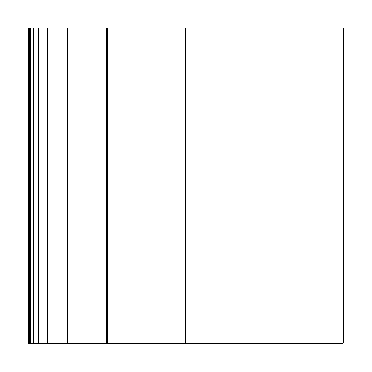
\begin{tikzpicture}
            \draw (0,0) -- (0,4);
            \draw (0,0) -- (4,0);
            \draw (4,4) -- (4,0);
            \draw (2,0) -- (2,4);
            \draw (1,0) -- (1,4);
            \draw (0.5,0) -- (0.5,4);
            \draw (0.25,0) -- (0.25,4);
            \draw (0.125,0) -- (0.125,4);
            \draw (0.0625,0) -- (0.0625,4);
            \draw (0.03125,0) -- (0.03125,4);
            \draw (0.015625,0) -- (0.015625,4);
        \end{tikzpicture}
        \caption{Conjunto $X$.}
        \label{fig:12_rel2}
    \end{figure}
    \noindent
    Si consideramos la aplicación $H:X\times [0,1]\to X$ dada por:
    \begin{equation*}
        H((x,y),t) = \left\{\begin{array}{ll}
                (x,(1-2t)y)& \text{si\ } 0\leq t\leq \nicefrac{1}{2}\\
                (2(1-t)x,0)& \text{si\ } \nicefrac{1}{2}\leq t\leq 1
        \end{array}\right. 
    \end{equation*}
    Tenemos que:
    \begin{itemize}
        \item $H$ está bien definida, pues:
            \begin{equation*}
                \left(x,\left(1-\frac{\nicefrac{1}{2}}{2}\right)y\right) = (x,(1-1)y) = (x,0) = \left(2\left(1-\frac{1}{2}\right)x,0\right) 
            \end{equation*}
        \item $H$ es claramente continua en $X\times [0,\nicefrac{1}{2}]$ y en $X\times [\nicefrac{1}{2},1]$, por lo que por el Lema del Pegado obtenemos que $H$ es continua.
        \item $H$ cumple que:
            \begin{equation*}
                H((x,y),0) = (x,y),\quad H((x,y),1) = (0,0)\qquad \forall (x,y)\in X
            \end{equation*}
    \end{itemize}
    Por lo que hemos probado que $\{(0,0)\}$ es retracto de deformación de $X$, luego $X$ es contráctil.
\end{ejercicio}

\begin{ejercicio}
    Sea $f:\mathbb{R}\to \mathbb{R}^+$ una función continua. Definimos el conjunto:
    \begin{equation*}
        S_f = \left\{(x,y,z)\in \mathbb{R}^3: x^2+y^2 = {(f(z))}^{2}\right\}
    \end{equation*}
    \begin{enumerate}[label=\alph*)]
        \item Estudia el conjunto $S_f\cap \{z=z_0\}$ con $z_0\in \mathbb{R}$.

            Fijado $z_0\in \mathbb{R}$, tenemos que:
            \begin{equation*}
                S_f \cap \{z=z_0\} = \left\{(x,y,z)\in \mathbb{R}^3 : x^2+y^2 = {(f(z_0))}^{2}\right\}
            \end{equation*}
            que se trata de una circunferencia de centro $(0,0,z_0)$ y de radio $f(z_0)$. Podemos interpretar $S_f$ como el sólido de revolución obtenido a partir de la gráfica de $f$.

        \item Demuestra que cualesquiera dos conjuntos $S_f$ son homeomorfos entre sí.

            Sea $f:\mathbb{R}\to \mathbb{R}^+$ una función continua, consideramos $\Phi:S_f\to \bb{S}^1\times \mathbb{R}$ dada por:
            \begin{equation*}
                \Phi(x,y,z) = \left(\frac{x}{\sqrt{x^2+y^2}}, \frac{y}{\sqrt{x^2+y^2}}, z\right)
            \end{equation*}
            Así como la aplicación $\Psi:\bb{S}^1\times \mathbb{R}\to S_f$ dada por:
            \begin{equation*}
                \Psi(x,y,z) = (f(z)x, f(z)y, z)
            \end{equation*}
            Es claro que $\Phi$ y $\Psi$ son continuas, así como que:
            \begin{align*}
                &\Phi(\Psi(x,y,z)) = \Phi(f(z)x, f(z)y, z) = \\ 
                &=\left(\frac{f(z)x}{\sqrt{{(f(z)x)}^{2} + {(f(z)y)}^{2}}}, \frac{f(z)y}{\sqrt{{(f(z)x)}^{2} + {(f(z)y)}^{2}}}, z\right)\\
                &=\left(\frac{f(z)x}{\sqrt{{(f(z))}^{2}(x^2+y^2)}}, \frac{f(z)y}{\sqrt{{(f(z))}^{2}(x^2+y^2)}}, z\right) =\left(\frac{f(z)x}{\sqrt{{(f(z))}^{2}}}, \frac{f(z)y}{\sqrt{{(f(z))}^{2}}}, z\right)\\
                &=\left(\frac{f(z)x}{f(z)}, \frac{f(z)y}{f(z)}, z\right) = (x,y,z) \qquad \forall (x,y,z)\in \bb{S}^1\times \mathbb{R} \\
                &\Psi(\Phi(x,y,z)) = \Psi\left(\frac{x}{\sqrt{x^2+y^2}}, \frac{y}{\sqrt{x^2+y^2}}, z\right)= \left(\frac{f(z)x}{\sqrt{x^2+y^2}}, \frac{f(z)y}{\sqrt{x^2+y^2}}, z\right) \\
                &= \left(\frac{\sqrt{x^2+y^2}\cdot x}{\sqrt{x^2+y^2}}, \frac{\sqrt{x^2+y^2}\cdot y}{\sqrt{x^2+y^2}}, z\right)  = (x,y,z) \qquad \forall (x,y,z)\in S_f
            \end{align*}
            Por lo que $\Phi$ es un homeomorfismo.
        \item Calcula el grupo fundamental de $S_f$.

            Dado $(x,y,z)\in S_f$, el homeomorfismo $\Phi$ anterior induce un isomorfismo:
            \begin{equation*}
                \Phi_\ast:\pi_1(S_f,(x,y,z)) \to \pi_1(\bb{S}^1\times \mathbb{R},\Phi(x,y,z))
            \end{equation*}
            Y como $\pi_1(\bb{S}^1\times \mathbb{R},\Phi(x,y,z))\cong \mathbb{Z}$, tenemos que $\pi_1(S_f,(x,y,z))\cong \mathbb{Z}$.
    \end{enumerate}
\end{ejercicio}

\begin{ejercicio}
    Prueba que $\mathbb{R}\times \left[0,+\infty\right[$ no es homeomorfo a $\mathbb{R}^2$. ¿Son del mismo tipo de homotopía?\\

        \noindent
        Por reducción al absurdo, si $\mathbb{R}\times \left[0,+\infty\right[$ fuera homeomorfo a $\mathbb{R}^2$, existiría un homeomorfismo $f:\mathbb{R}\times \left[0,+\infty\right[\to \mathbb{R}^2$, por lo que la restricción de $f$ \newline$f\big|_{(\mathbb{R}\times \left[0,+\infty\right[)\setminus\{(0,0)\}}:(\mathbb{R}\times \left[0,+\infty\right[)\setminus\{(0,0)\}\to \mathbb{R}^2\setminus\{f(0,0)\}$ seguiría siendo un homeomorfismo, que induciría un isomorfismo entre sus grupos fundamentales.

                        Sin embargo, $(\mathbb{R}\times \left[0,+\infty\right[)\setminus\{(0,0)\}$ es un conjunto estrellado, luego es simplemente conexo y $\mathbb{R}^2\setminus\{f(0,0)\}$ es homeomorfo a $\bb{S}^1$, que tiene $\mathbb{Z}$ como grupo fundamental, por lo que no pueden ser homeomorfos, contradicción que viene de suponer la que $\mathbb{R}\times \left[0,+\infty\right[$ y $\mathbb{R}^2$ son homeomorfos.\\

        \noindent
        Sí son del mismo tipo de homotopía. Para verlo, veamos que $\mathbb{R}\times \left[0,+\infty\right[$ es un retracto de deformación de $\mathbb{R}^2$, ya que definiendo $H:\mathbb{R}^2\times [0,1]\to \mathbb{R}^2$ dada por:
            \begin{equation*}
                H((x,y),t) = \left\{\begin{array}{ll}
                        (x,y) & \text{si\ } (x,y)\in \mathbb{R}\times \left[0,+\infty\right[ \\
                        (x, (1-t)y) & \text{si\ } (x,y)\in \mathbb{R}\times \left]-\infty, 0\right]
                \end{array}\right. 
            \end{equation*}
            Tenemos que:
            \begin{itemize}
                \item $H$ está bien definida, puesto que:
                    \begin{equation*}
                        (x,0) = (x,(1-t)0), \qquad \forall t\in [0,1]
                    \end{equation*}
                \item $H$ es continua, puesto que es continua en los cerrados $\mathbb{R}\times \left[0,+\infty\right[\times [0,1]$, $\mathbb{R}\times \left]-\infty,0\right]\times [0,1]$, luego podemos aplicar el Lema del Pegado.
                \item Se verifica que:
                    \begin{multline*}
                        H((x,y),0) = (x,y), \quad H((x,y),1) \in \mathbb{R}\times \left[0,+\infty\right[, \quad H((a,b),1) = (a,b) \\
                            \forall (x,y)\in \mathbb{R}^2, \quad \forall (a,b)\in \mathbb{R}\times \left[0,+\infty\right[
                    \end{multline*}
            \end{itemize}
            Por lo que $\mathbb{R}\times \left[0,+\infty\right[$ es retracto de deformación de $\mathbb{R}^2$ para $r:\mathbb{R}^2\to \mathbb{R}\times \left[0,+\infty\right[$ dada por $r(x,y) = H((x,y),1)$, que induce un isomorfismo entre grupos fundamentales $r_\ast:\pi_1(\mathbb{R}^2,(x,y))\to \pi_1(\mathbb{R}\times \left[0,+\infty\right[, r(x,y))\quad \forall (x,y)\in \mathbb{R}^2$, luego $\mathbb{R}\times \left[0,+\infty\right[$ y $\mathbb{R}^2$ son del mismo tipo de homotopía.
\end{ejercicio}

\begin{ejercicio}
    Sea $S$ un subespacio afín de $\mathbb{R}^n$ de dimensión $k\leq n-2$. Calcula $\pi_1(\mathbb{R}^n\setminus S)$.\\

    \noindent
    Estudiemos ejemplos particulares para obtener intuición:
    \begin{itemize}
        \item Para $n=2$, si $S$ es un subespacio afín de $\mathbb{R}^2$ de dimensión $0$ ($S$ se reduce a un punto), entonces:
            \begin{equation*}
                \pi_1(\mathbb{R}^2\setminus S) \cong \mathbb{Z}
            \end{equation*}
            Ya que $\mathbb{R}^2\setminus S \cong \mathbb{R}^2\setminus \{(0,0)\}$ y este último tiene por retracto de deformación a $\bb{S}^1$.
            \begin{figure}[H]
                \centering
            \begin{tikzpicture}
                % Ejes coordenados
                \draw[-Stealth] (-1.4,0) -- (1.4,0) node[right] {};
                \draw[-Stealth] (0,-1.4) -- (0,1.4) node[above] {};

                % Punto (0,0) quitado: círculo no relleno
                \draw[fill=white,thick] (0,0) circle (0.05);

                % Circunferencia de radio 1
                \draw[thick] (0,0) circle (1);
            \end{tikzpicture}
            \end{figure}
        \item Para $n=2$, si $S$ es un subespacio afín de $\mathbb{R}^3$ de dimensión:
            \begin{itemize}
                \item $dim S = 0$, entonces:
                    \begin{equation*}
                        \pi_1(\mathbb{R}^3\setminus S) = \{1\}
                    \end{equation*}
                    Ya que $\mathbb{R}^3\setminus S \cong \mathbb{R}^3\setminus \{(0,0,0)\}$ y este último tiene por retracto de deformación a $\bb{S}^2$.
                \item $dim S = 1$, entonces:
                    \begin{equation*}
                        \pi_1(\mathbb{R}^3\setminus S) \cong \mathbb{Z}
                    \end{equation*}
                    Ya que $\mathbb{R}^3\setminus S$ tiene por retracto de deformación un conjunto homeomorfo a $\bb{S}^1\times \mathbb{R}$.
            \end{itemize}
    \end{itemize}
    Comenzando ahora la prueba formal, sea $S$ un subespacio afín de $\mathbb{R}^n$ de dimensión $k \leq n-2$, tenemos entonces que $S$ es homeomorfo al subespacio afín $\cc{S}$, dado por las ecuaciones\footnote{Como es de dimensión $k$ en $\mathbb{R}^n$ ha de tener $n-k$ ecuaciones.}:
    \begin{equation*}
        \left\{\begin{array}{l}
            x_1 = 0 \\
            \vdots \\
            x_{n-k} = 0
        \end{array}\right.
    \end{equation*}
    De esta forma, tenemos que:
    \begin{equation*}
        \mathbb{R}^n\setminus \cc{S} = (\mathbb{R}^{n-k}\setminus \{(0,0,\ldots, 0)\})\times \mathbb{R}^k
    \end{equation*}
    Por lo que:
    \begin{equation*}
        \pi_1(\mathbb{R}^n\setminus S) = \pi_1(\mathbb{R}^n\setminus \cc{S}) = \pi_1\left(\mathbb{R}^{n-k}\setminus \{(0,0,\ldots,0)\}\right) \times \pi_1(\mathbb{R}^k) \cong \pi_1\left(\mathbb{R}^{n-k}\setminus \{(0,0,\ldots,0)\}\right)
    \end{equation*}
    Y tenemos que:
    \begin{equation*}
        \pi_1(\mathbb{R}^n\setminus S)\cong \pi_1\left(\mathbb{R}^{n-k}\setminus \{(0,\ldots,0)\}\right) \cong \left\{\begin{array}{ll}
            \mathbb{Z} & \text{si\ } n-k=2 \\
             \{1\}& \text{si\ } n-k >2
        \end{array}\right. 
    \end{equation*}
\end{ejercicio}

\begin{ejercicio}
    Prueba que si $X$ es de Hausdorff y $A\subseteq X$ es un retracto de $X$, entonces $A$ es cerrado en $X$. Deduce que una bola abierta en $\mathbb{R}^n$ no es un retracto de $\mathbb{R}^n$. ¿Lo es una bola cerrada?\\

    \noindent
    Para probar que $A$ es cerrado, veamos que $X\setminus A$ es abierto. Para ello, sea $x\in X\setminus A$, tendremos entonces que $a = r(x) \neq x$. Como $X$ es de Hausdorff, podemos encontrar abiertos $U_x, U_a$ con:
    \begin{equation*}
        x\in U_x, \qquad a\in U_a,\qquad U_x\cap U_a = \emptyset 
    \end{equation*}
    Si consideramos $W=U_x\cap r^{-1}(U_a)$, tenemos que $W$ es abierto como intersección de dos abiertos, así como que $x\in W$. Si existiera $b\in W\cap A$, tendríamos entonces que $b\in U_x\cap r^{-1}(U_a)\cap A$, por lo que:
    \begin{equation*}
        U_x\ni b = r(b) \in U_a \Longrightarrow b\in U_x\cap U_a
    \end{equation*}
    \underline{contradicción} que viene de suponer que $W\cap A \neq \emptyset $, luego $x\in W\subseteq X\setminus A$, de donde $X\setminus A$ es abierto.\\

    \noindent
    Sea $B(x,r)\subseteq \mathbb{R}^n$ una bola abierta para ciertos puntos $x\in \mathbb{R}^n$, $r\in \mathbb{R}^+$, esta no puede ser un retracto de $\mathbb{R}^n$ puesto que no es cerrada, ya que si tomamos como $t_n$ una sucesión de puntos del intervalo $\left[0,r\right[$ convergente a $r$ (por ejemplo $r-\frac{1}{n}$), tenemos entonces que $\left\{x+\frac{x}{\|x\|}t_n\right\}$ es una sucesión de puntos de $B(x,r)$:
        \begin{equation*}
            \left\|x+\frac{x}{\|x\|}t_n - x\right\| = \frac{t_n\|x\|}{\|x\|} = t_n < r
        \end{equation*}
        convergente a $x+r\frac{x}{\|x\|}$, con:
        \begin{equation*}
            \left\|x+r\frac{x}{\|x\|}-x\right\| = \frac{r\|x\|}{\|x\|} = r \Longrightarrow x+r\frac{x}{\|x\|}\notin B(x,r)
        \end{equation*}

    \noindent
    Sea ahora $\overline{B}(x,r)\subseteq \mathbb{R}^n$  una bola cerrada para ciertos puntos $x\in \mathbb{R}^n$, $r\in \mathbb{R}^+$, podemos construir la aplicación $r:\mathbb{R}^n\to \overline{B}(x,r)$ dada por:
    \begin{equation*}
        r(y) = \left\{\begin{array}{ll}
            y & \text{si\ } y\in \overline{B}(x,r) \\
            c(y) & \text{si\ } y\in \mathbb{R}^n\setminus B(x,r)
        \end{array}\right. 
    \end{equation*}
    donde $c(y)$ es la aplicación que a cada punto $y$ le hace corresponder aquel punto de la semirrecta con origen en $x$ y que pasa por $y$ con módulo $r$. En teoría vimos en un ejemplo parecido que la aplicación $c$ era continua, por lo que aplicando el Lema del Pegado vemos que $r$ es continua, así como que:
    \begin{equation*}
        r(y) = y \qquad \forall y\in \overline{B}(x,r)
    \end{equation*}
    por lo que $\overline{B}(x,r)$ es un retracto de $\mathbb{R}^n$.
\end{ejercicio}

\begin{ejercicio}
    En este ejercicio demostraremos que \textit{un abierto de $\mathbb{R}^2$ no puede ser homeomorfo a un abierto de $\mathbb{R}^n$ si} $n\geq 3$. Supongamos que $f:U\to V$ es un homeomorfismo entre abiertos no vacíos $U\subset \mathbb{R}^n$ y $V\subset \mathbb{R}^2$ con $n\geq 3$.
    \begin{enumerate}[label=\alph*)]
        \item Prueba que existen bolas abiertas $B_1\subset U$ y $B_2,B_2'\subset V$ (estas últimas con el mismo centro $y_0\in \mathbb{R}^2$) tales que $\overline{B_2'}\subset f(\overline{B_1})\subset \overline{B_2}$.
        \item Si $i:\overline{B_2'}\setminus \{y_0\}\to \overline{B_2}\setminus \{y_0\}$ es la inclusión, deduce de $a)$ que el homomorfismo inducido en cualquier punto $i_\ast$ es trivial.
        \item Prueba que $\overline{B_2'}\setminus \{y_0\}$ es un retracto de deformación de $\overline{B_2}\setminus \{y_0\}$. Concluye que $i_\ast$ es un isomorfismo no trivial, lo que contradice $b)$.
    \end{enumerate}

    \noindent
    \textbf{Solución.}
    \begin{enumerate}[label=\alph*)]
        \item Prueba que existen bolas abiertas $B_1\subset U$ y $B_2,B_2'\subset V$ (estas últimas con el mismo centro $y_0\in \mathbb{R}^2$) tales que $\overline{B_2'}\subset f(\overline{B_1})\subset \overline{B_2}$.

            Fijado cualquier $y_0\in V$, como $V$ es abierto ha de existir una bola abierta $B_2$ centrada en $y_0$ y contenida en $V$. Si consideramos $x_0 = f^{-1}(y_0)$, como $f$ es continua el conjunto $f^{-1}(B_2)$ será también abierto, con $x_0\in f^{-1}(B_2)$, por lo que ha de existir una bola abierta $B_1$ centrada en $x_0$ y contenida en $f^{-1}(B_2)$. Como $f$ es continua, ha de cumplirse que:
            \begin{equation*}
                f(\overline{B_1})\subseteq \overline{f(B_1)} \subseteq \overline{B_2}
            \end{equation*}
            Si consideramos ahora $f(B_1)$, como $B_1$ estaba centrada en $x_0$ tenemos que $y_0 \in f(B_1)$ y como $f$ es una aplicación abierta por ser un homeomorfismo, $f(B_1)$ será también un conjunto abierto, por lo que podemos encontrar una bola abierta $B_2'$ centrada en $y_0$ y de modo que:
            \begin{equation*}
                \overline{B_2'} \subseteq f(B_1) \subseteq f(\overline{B_1})
            \end{equation*}
        \begin{figure}[H]
            \centering
            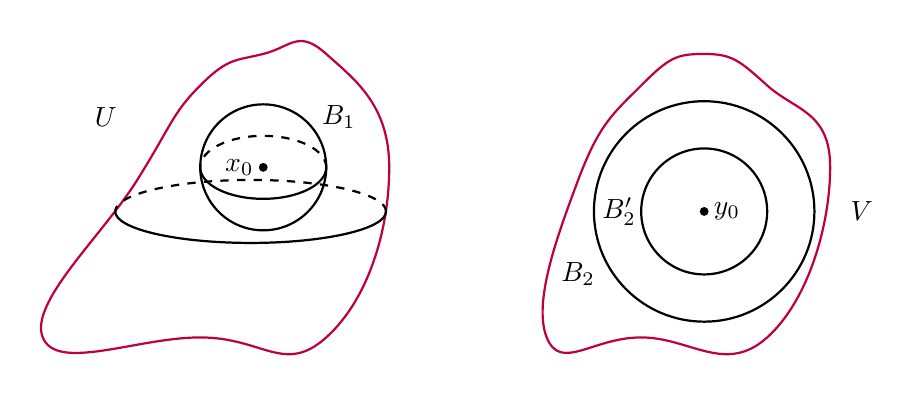
\begin{tikzpicture}[scale=0.8]
                \shorthandoff{>}
                % Abierto
                \draw[purple, thick] plot[smooth cycle, tension=0.8] coordinates {
                    (-1,0.5) (0,2) (1,2.5) (2,2.5) (3, 0.7) (2,-2) (0,-2) (-2.5,-2)
                };
                \draw[thick, dashed] (2.95,0) arc (0:180:2.15 and 0.5);
                \draw[thick] (2.95,0) arc (0:-180:2.15 and 0.5);
                \fill (-1.5,1.5) node{$U$};

                % Esfera chica
                \draw[thick] (1,0.7) circle [radius=1];
                \fill (1,0.7) circle(2pt) node[left]{$x_0$};
                \draw[thick, dashed] (2,0.7) arc (0:180:1 and 0.5);
                \draw[thick] (2,0.7) arc (0:-180:1 and 0.5);
                \fill (2.2,1.5) node{$B_1$};

                % Circunferencia
                \draw[thick] (8,0) circle [radius=1.75];
                \draw[thick] (8,0) circle [radius=1];

                % Abierto V
                \draw[purple, thick] plot[smooth cycle, tension=0.8] coordinates {
                    (6,0.5) (7,2) (8,2.5) (9,2) (10, 0.7) (9,-2) (7,-2) (5.5,-2)
                };
                \fill (10.5,0) node{$V$};
                \fill (6,-1) node{$B_2$};
                \fill (6.65,0) node{$B_2'$};
                \fill (8,0) circle(2pt) node[right]{$y_0$};
            \end{tikzpicture} 
        \end{figure}

        \item Si $i:\overline{B_2'}\setminus \{y_0\}\to \overline{B_2}\setminus \{y_0\}$ es la inclusión, deduce de $a)$ que el homomorfismo inducido en cualquier punto $i_\ast$ es trivial.

            \begin{description}
                \item [Opción 1.] Fijado $z_0\in \overline{B_2'}\setminus \{y_0\}$, consideramos un lazo $\alpha\in \Omega(\overline{B_2'}\setminus \{y_0\})$ y consideramos el lazo $f^{-1}\circ \alpha$, que está basado en $f^{-1}(z_0)$ y cumple que:
                    \begin{equation*}
                        Im(f^{-1}\circ \alpha) \subseteq f^{-1}(\overline{B_2'}\setminus y_0) \subseteq \overline{B_1}\setminus \{x_0\}
                    \end{equation*}
                    Como $\pi_1(\overline{B_1}\setminus\{x_0\},f^{-1}(z_0))$ es trivial (por tener $\overline{B_1}\setminus \{x_0\}$ un retracto de deformación homeomorfo a $\bb{S}^n$)  tenemos entonces que $[f^{-1}\circ \alpha] = [\varepsilon_{f^{-1}(z_0)}]$, por lo que existe una homotopía por arcos $H$ de forma que:
                    \begin{equation*}
                        H(t,0) = f^{-1}(z_0), \qquad H(t,1) = (f^{-1}\circ \alpha)(t) \qquad \forall t\in [0,1]
                    \end{equation*}
                    Finalmente, observamos que $f\circ f^{-1}\circ \alpha = \alpha$ y que $f\circ H$ es una homotopía que cumple:
                    \begin{equation*}
                        (f\circ H)(t,0) = z_0, \qquad (f\circ H)(t,1) = \alpha(t) \qquad \forall t\in [0,1]
                    \end{equation*}
                    Con:
                    \begin{equation*}
                        Im(f\circ H)\subseteq f(\overline{B_1}\setminus\{x_0\})\subseteq \overline{B_2}\setminus \{y_0\}
                    \end{equation*}
                    Por lo que $i_\ast([\alpha]) = [\alpha]_{\overline{B_2}\setminus \{y_0\}} = [\varepsilon_{z_0}]$.
                \item [Opción 2.] Como $\overline{B_2'}\setminus \{y_0\}\subseteq f(\overline{B_1})\setminus\{x_0\}$, podemos considerar:
                    \Func{\varphi}{\overline{B_2'}\setminus\{y_0\}}{\overline{B_1}\setminus\{x_0\}}{x}{f^{-1}(x)}
                    que será una aplicación continua, como restricción de $f^{-1}:V\to U$ en dominio y codominio. Análogamente, como $f(\overline{B_1})\setminus\{x_0\}\subseteq \overline{B_2'}\setminus\{y_0\}$, podemos considerar:
                    \Func{\phi}{\overline{B_1}\setminus\{x_0\}}{\overline{B_2}\setminus\{y_0\}}{y}{f(y)}
                    que también será una aplicación continua, como restricción de $f$ en dominio y codominio. Observamos que de esta forma tenemos:
                    \begin{equation*}
                        \phi(\varphi(x)) = \phi(f^{-1}(x)) = f(f^{-1}(x)) = x = i(x) \qquad \forall x\in \overline{B_2'}\setminus\{y_0\}  
                    \end{equation*}
                    Por lo que el siguiente diagrama es conmutativo:
                    \begin{figure}[H]
                        \centering
                        \shorthandoff{""}
                        \begin{tikzcd}
                            \overline{B_2'}\setminus\{y_0\} \arrow[r, "\varphi"] \arrow[rr, "i"', hook, bend right] & \overline{B_1}\setminus\{x_0\} \arrow[r, "\phi"] & \overline{B_2}\setminus\{y_0\}
                        \end{tikzcd}
                        \shorthandon{""}
                    \end{figure}
                    \noindent
                    Si inducimos ahora el diagrama a grupos fundamentales para un punto $z_0\in \overline{B_2'}\setminus\{y_0\}$ arbitrario, obtenemos el diagrama:
                    \begin{figure}[H]
                        \centering
                        \shorthandoff{""}
                        \begin{tikzcd}
                            {\pi_1(\overline{B_2'}\setminus\{y_0\},z_0)} \arrow[r, "\varphi_\ast"] \arrow[rr, "i_\ast"', hook, bend right] & {\pi_1(\overline{B_1}\setminus\{x_0\},\varphi(z_0))} \arrow[r, "\phi_\ast"] & {\pi_1(\overline{B_2}\setminus\{y_0\},z_0)}
                        \end{tikzcd}
                        \shorthandon{""}
                    \end{figure}
                    Y como $\pi_1(\overline{B_1}\setminus \{x_0\},\varphi(z_0))$ es trivial por tener $\overline{B_1}\setminus\{x_0\}$ un retracto de deformación homeomorfo a $\bb{S}^n$, obtenemos por tanto que $i_\ast$ es trivial.
            \end{description}
        \item Prueba que $\overline{B_2'}\setminus \{y_0\}$ es un retracto de deformación de $\overline{B_2}\setminus \{y_0\}$. Concluye que $i_\ast$ es un isomorfismo no trivial, lo que contradice $b)$.

            Supuesto que $\overline{B_2'}\setminus \{y_0\}$ es una bola cerrada punteada\footnote{Es decir, a la que hemos quitado el centro} de radio $r\in \mathbb{R}^+$, podemos definir la aplicación $H:(\overline{B_2}\setminus\{y_0\})\times [0,1]\to \overline{B_2}\setminus \{y_0\}$ dada por:
            \begin{equation*}
                H(x,t) = \left\{\begin{array}{ll}
                    x & \text{si\ } x\in \overline{B_2'}\setminus \{y_0\} \\
                    (1-t)x + tr\cdot  \frac{x}{\|x\|_2}& \text{si\ } x\notin \overline{B_2'}\setminus \{y_0\}
                \end{array}\right. 
            \end{equation*}
            Que es continua y verifica: 
            \begin{gather*}
                H(x,0) = x, \qquad H(x,1) \in \overline{B_2'}\setminus \{y_0\} \qquad \forall x\in \overline{B_2}\setminus \{y_0\} \\
                H(y,1) =  y \qquad \forall x\in \overline{B_2'}\setminus \{y_0\}
            \end{gather*}
            Por tanto, el grupo fundamental de $\overline{B_2'}\setminus \{y_0\}$ coincide (en cualquier punto $z_0$) con el grupo fundamental de $\overline{B_2}\setminus \{y_0\}$, lo que contradice que $i_\ast$ sea trivial.
    \end{enumerate}
\end{ejercicio}

\begin{ejercicio}
    Demuestra que el sistema de ecuaciones:
    \begin{equation*}
        \left\{\begin{array}{l}
            x-\arctg(x^2-y^3) = 2 \\
            \cos(x) + \sen(xy^3) + e^x + e^{y^2} + \dfrac{1}{y} = -5
        \end{array}\right.
    \end{equation*}
    tiene al menos una solución en $\mathbb{R}^2$.\\

    \noindent
    Si llamamos a dicho sistema de ecuaciones por $(\ast)$, vemos que este es equivalente al siguiente sistema de ecuaciones (al que llamamos $(\ast\ast)$) cuando $y\neq 0$:
    \begin{equation*}
        \left\{\begin{array}{l}
            x = 2 + \arctg(x^2-y^3) \\
            y = \dfrac{-1}{5+\cos(x) + \sen(xy^3) + e^x + e^{y^2}}
        \end{array}\right.
    \end{equation*}
    Definimos $F:\mathbb{R}^2\to \mathbb{R}^2$ dada por:
    \begin{equation*}
        F(x,y) = \left(2 + \arctg(x^2-y^3), \dfrac{-1}{5+\cos(x) + \sen(xy^3) + e^x + e^{y^2}}\right)
    \end{equation*}
    Observemos que el denominador de la segunda componente no se anula, ya que $e^x,e^{y^2}>0$ para todo $(x,y)\in \mathbb{R}^2$ así como que $5+\cos(x)+\sen(xy^3)>0$ para todo $(x,y)\in \mathbb{R}^2$, por ser $|\cos(x)|,|\sen(xy^3)|\leq 1$. Por tanto, tenemos que $F$ es continua, ya que cada una de sus componentes es una función continua.\\

    \noindent
    Ahora, fijado $(x,y)\in \mathbb{R}^2$, si escribimos $F=(F_1,F_2)$, tenemos que $|F_1(x,y)| \leq 2+\frac{\pi}{2}$, así como que $|F_2(x,y)|<\nicefrac{1}{3}$, por lo que deducimos que $F$ está acotada, es decir, existe $R\in \mathbb{R}^+$ de forma que:
    \begin{equation*}
        \|F(x,y)\|_2 \leq R \qquad \forall (x,y)\in \mathbb{R}^2
    \end{equation*}
    Por lo que podemos considerar la aplicación restringida $\tilde{F}:\overline{B}(0,R)\to \overline{B}(0,R)$ dada por $\tilde{F}(x) = F(x)$. Si aplicamos el Teorema del Punto fijo de Brouwer, obtenemos que existe $(x_0,y_0)\in \overline{B}(0,R)$ de forma que:
    \begin{equation*}
        \tilde{F}(x_0,y_0) = (x_0,y_0)
    \end{equation*}
    Por lo que hemos encontrado una solución al sistema $(\ast\ast)$. Más aún, observemos que como $F_2(x_0,y_0)<0$ debe ser $y_0<0$, en particular $y_0\neq 0$, por lo que $(x_0,y_0)$ tamién es solución del sistema $(\ast)$.
\end{ejercicio}

\begin{ejercicio}
    Sean $M$ una matriz cuadrada real de orden 3 por 3 cuyas entradas son números reales positivos
    y $f:\mathbb{R}^3\to \mathbb{R}^3$ la aplicación lineal $f(v)=Mv$. Demuéstrese que:
    \begin{enumerate}[label=\alph*)]
        \item El conjunto $A=\{(x,y,z)\in \bb{S}^2:x,y,z\geq 0\}$ es homeomorfo al disco cerrado $\overline{\bb{D}}$.

            Es decir, queremos probar que la parte de la esfera $\bb{S}^2$ que se encuentra en el primer octante es homeomorfo a $\overline{\bb{D}}$. Para ello, lo que haremos primero será considerar el conjunto:
            \begin{equation*}
                C = \{(x,y,0)\in \mathbb{R}^3 : \|(x,y,0)\|_2 \leq 1 \ \land\  x,y\geq 0\}
            \end{equation*}
            \begin{figure}[H]
                \centering
                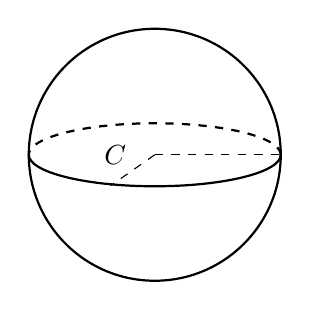
\begin{tikzpicture}[scale=0.8]
                    \shorthandoff{>}
                    % Esfera
                    \draw[thick] (0,0) circle [radius=2];
                    \draw[thick, dashed] (2,0) arc (0:180:2 and 0.5);
                    \draw[thick] (2,0) arc (0:-180:2 and 0.5);

                    % \draw[dashed] (0,2) -- (0,0);
                    \draw[dashed] (0,0) -- (2,0);
                    \draw[dashed] (0,0) -- (-0.7,-0.49);

                    \fill (-0.3,0) node[left] {$C$};
                \end{tikzpicture} 
            \end{figure}
            Y vemos que si consideramos la función que a cada punto de $C$ le asigna la altura de la esfera en la parte superior:
            \Func{F}{C}{\bb{R}}{(x,y)}{\sqrt{1-x^2-y^2}}
            Tenemos que $A = Gr(F)$, con $F$ una función continua, por lo que $A$ y $C$ son homeomorfos. Finalmente tenemos que probar que $C$ y $\overline{\bb{D}}$ son homeomorfos. Para ello, es sencillo dar primero un homeomorfismo $h:\delta C\to \bb{S}^1$ (hágase). Ahora, fijado $p_0\in C^\circ$ cada punto $c\in C$ puede expresarse como:
            \begin{equation*}
                c = (1-t)p_0 + tx
            \end{equation*}
            para cierto $t\in [0,1]$ y $x\in \delta C$. Podemos hacer corresponder dicho punto mediante una aplicación $p:C\to \overline{\bb{D}}$ a:
            \begin{equation*}
                c = (1-t)p_0 + tx \longmapsto (1-t)\cdot 0 + th(x) = th(x)
            \end{equation*}
            es claro que $p$ es continua y biyectiva, y como va de un conjunto cerrado a un Hausdorff será también una aplicación cerrada, por lo que $p$ es un homeomorfismo.
        \item La aplicación $g:A\to \bb{S}^2$ dada por $g(v) = \frac{f(v)}{|f(v)|}$ está bien definida y $g(A)\subset A$.

            Recordamos que según el enunciado tenemos que $f(v) = Mv$ con $M = (m_{i,j})_{i,j}$ de forma que $m_{i,j}> 0$ para $i,j\in \{1,2,3\}$. Dado $v\in A$, tendremos que $v = (v_1, v_2, v_3)$ con $v_1,v_2,v_3\geq 0$. De esta forma, podemos obtener $f(v)$ calculando:
            \begin{equation*}
                f(v) = Mv = \left(\begin{array}{ccc}
                    m_{1,1} & m_{1,2} & m_{1,3} \\
                    m_{2,1} & m_{2,2} & m_{2,3} \\
                    m_{3,1} & m_{3,2} & m_{3,3} 
                \end{array}\right) \left(\begin{array}{ccc}
                    v_1 \\
                    v_2 \\
                    v_3 
                \end{array}\right) = \left(\begin{array}{ccc}
                     m_{1,1} v_1 + m_{1,2}v_2 + m_{1,3}v_3 \\
                     m_{2,1} v_1 + m_{2,2}v_2 + m_{2,3}v_3 \\
                     m_{3,1} v_1 + m_{3,2}v_2 + m_{3,3}v_3 
                \end{array}\right)
            \end{equation*}
            Observamos que para obtener $f(v) = 0$ tendríamos que tener (como $m_{i,j}>0$ y $v_1,v_2,v_3\geq 0$) que $v_1 = v_2 = v_3 = 0$, pero como $v\in A\subseteq \bb{S}^2$ dicha situación es imposible, por lo que el denominador de la función $g$ nunca se anula. Más aún, $|g(v)| = 1$ para todo $v\in A$, por lo que $g$ está bien definida.

            Finalmente, similar a lo que hemos comentado ya, como $m_{i,j}>0$ para todo $i,j\in \{1,2,3\}$ y $v_1,v_2,v_3\geq 0$ tendremos por tanto (observando las cuentas que hacemos para calcular $f(v)$) que $f(v)\in A$.
        \item $f$ tiene un valor propio real y positivo.

            Usando el apartado $b)$ tenemos que podemos restringir $g$ en codominio, obteniendo una aplicación continua $g:A\to A$. Si usamos el apartado $a)$, existe $h:\overline{\bb{D}}\to A$ homeomorfismo, con lo que la aplicación $h^{-1}\circ g\circ h:\overline{\bb{D}}\to \overline{\bb{D}}$ es continua. Por el Teorema del punto fijo de Brouwer, existe $x_0\in \overline{\bb{D}}$ de forma que:
            \begin{equation*}
                (h^{-1}\circ g\circ h)(x_0) = x_0 \quad\Longrightarrow\quad g(h(x_0)) = h(x_0)
            \end{equation*}
            Por lo que tomando $z_0 = h(x_0)\in A$ obtenemos que:
            \begin{equation*}
                \frac{f(z_0)}{|f(z_0)|} = g(z_0) = z_0 \quad\Longrightarrow\quad f(z_0) =|f(z_0)|\cdot  z_0
            \end{equation*}
            De esta forma, hemos probado que $|f(z_0)|$ es un valor propio real y positivo de $f$.
    \end{enumerate}
\end{ejercicio}

\begin{ejercicio}
    Teorema de Lusternik-Schnirelmann. Demuestra que si $\bb{S}^2$ es la unión de tres subconjuntos cerrados $C_1,C_2,C_3$, entonces alguno de ellos contiene dos puntos antípodas. Para ello prueba que la función $f:\bb{S}^2\to \bb{R}^2$ dada por
    \begin{equation*}
        f(x) = (dist(x,C_1), dist(x,C_2))
    \end{equation*}
    tiene un punto $x_0\in \bb{S}^2$ tal que $f(x_0) = f(-x_0)$, donde $dist(\cdot ,\cdot )$ denota la función distancia en $\mathbb{R}^3$.\\

    \noindent
    Sean $C_1,C_2,C_3$ tres subconjuntos cerrados de $\bb{S}^2$ tales que:
    \begin{equation*}
        C_1\cup C_2\cup C_3 = \bb{S}^2
    \end{equation*}
    definimos la aplicación $f:\bb{S}^2\to \mathbb{R}^2$ dada por:
    \begin{equation*}
        f(x) = (dist(x,C_1), dist(x,C_2) \qquad \forall x\in \bb{S}^2
    \end{equation*}

    donde\footnote{Observemos que cada $C_i$ es compacto en $\mathbb{R}^3$.}:
    \begin{equation*}
        dist(x,C_i) = \min\{d(x,c) : c\in C_i\} \qquad i \in \{1,2,3\}
    \end{equation*}

    como cada aplicación $x\mapsto dist(x,C_i)$ es continua, tenemos que la aplicación $f$ es continua, y si aplicamos el Teorema de Borsuk-Ulam tenemos que $\exists x_0\in \bb{S}^2$ de forma que:
    \begin{equation*}
        (dist(x_0,C_1),dist(x_0,C_2)) = f(x_0) = f(-x_0)= (dist(-x_0,C_1),dist(-x_0,C_2))
    \end{equation*}

    de donde:
    \begin{equation*}
        dist(x_0,C_1) = dist(-x_0,C_1), \qquad dist(x_0,C_2) = dist(-x_0,C_2)
    \end{equation*}

    distinguimos casos:
    \begin{itemize}
        \item Si $dist(x_0,C_1), dist(x_0,C_2)>0$, tenemos entonces que tanto $x_0$ como $-x_0$ están en $C_3$.
        \item Si $dist(x_0,C_1) =0$, tenemos que $x_0,-x_0\in C_1$.
        \item Si $dist(x_0,C_2) =0$, tenemos que $x_0,-x_0\in C_2$.
    \end{itemize}
\end{ejercicio}

\begin{ejercicio}
    Calcula $\pi_1(X)$ en los siguientes casos:
    \begin{enumerate}[label=\alph*)]
        \item $X=\bb{S}^2 \cup (\bb{D}\times \{0\})$.

            Tenemos el conjunto de la Figura:
            \begin{figure}[H]
                \centering
                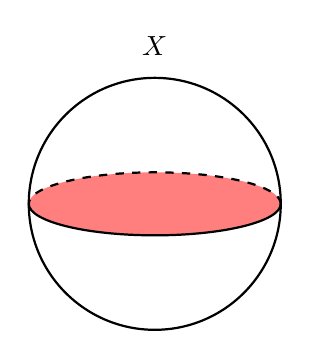
\begin{tikzpicture}[scale=0.8]
                    \shorthandoff{>}

                    \fill[red, opacity=0.5] (0,0) ellipse (2 and 0.5);

                    \draw[thick] (0,0) circle [radius=2];
                    \draw[thick, dashed] (2,0) arc (0:180:2 and 0.5);
                    \draw[thick] (2,0) arc (0:-180:2 and 0.5);

                    \node at (0,2.5) {$X$};

                \end{tikzpicture}
            \end{figure}

            Si tomamos los conjuntos:
            \begin{equation*}
                U = X\setminus \{(0,0,1)\}, \qquad V = X\setminus \{(0,0,-1)\}
            \end{equation*}
            Tenemos que:
            \begin{itemize}
                \item Claramente $X = U\cup V$.
                \item $U$ y $V$ son abiertos, ya que como estamos trabajando en un espacio métrico, los conjuntos unitarios son cerrados.
                \item Es claro que $U$ es homeomorfo a $V$ (basta considerar una rotación), y tenemos que $U$ es la unión de $\bb{S}^2\setminus \{(0,0,1)\}$, que es homeomorfo a $\mathbb{R}^2$ luego arcoconexo, con $\bb{D}\times \{0\}$, que claramente es arcoconexo, y estos dos conjuntos se cortan en al menos un punto (como por ejemplo el $(1,0,0)$), por lo que $U$ es arcoconexo y $V$ también por ser homeomorfo a $V$.
                \item $U\cap V$ es arcoconexo, ya que puede verse como la unión de los conjuntos:
                    \begin{equation*}
                        (\bb{S}^2\cap (\mathbb{R}^2\times \mathbb{R}^+_0))\cup \bb{D}\times \{0\}, \qquad 
                        (\bb{S}^2\cap (\mathbb{R}^2\times \mathbb{R}^-_0))\cup \bb{D}\times \{0\}
                    \end{equation*}
                    Ambos homeomorfos a $\bb{S}^2\setminus \{(0,0,1)\}$, que es arcoconexo, por lo que los dos conjuntos son arcoconexos y su unión también lo es, pues su intersección es $\bb{D}\times \{0\}$, que es arcoconexo.
            \end{itemize}
            Ahora, vemos que:
            \begin{itemize}
                \item Los grupos fundamentales de $U$ y de $V$ coinciden, pues ambos son homeomorfos.
                \item $U$ tiene como retracto de deformación el conjunto:
                    \begin{equation*}
                        U_1 = \{(x,y,z)\in \bb{S}^2 : z\leq 0\} \cup (\bb{D}\times \{0\})
                    \end{equation*}
                    Que es homeomofo a $\bb{S}^2$:
                    \begin{figure}[H]
                        \centering
                        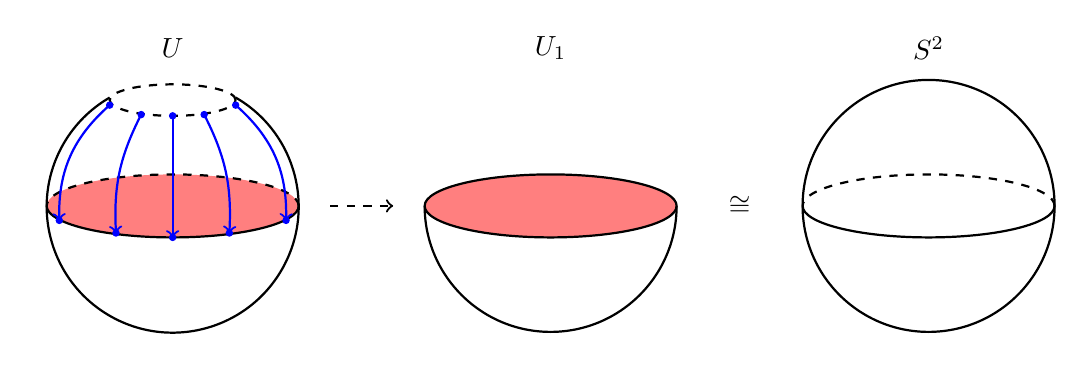
\begin{tikzpicture}[scale=0.8]
                            \shorthandoff{>}

                            \begin{scope}[shift={(-2,0)}]
                                \node at (0,2.5) {$U$};

                                % Color radio medio
                                \fill[red, opacity=0.5] (0,0) ellipse (2 and 0.5);

                                % Radio medio
                                \draw[thick, dashed] (2,0) arc (0:180:2 and 0.5);
                                \draw[thick] (2,0) arc (0:-180:2 and 0.5);

                                % Agujero superior
                                \draw[thick, dashed] (0,1.68) ellipse (1 and 0.25);
                                \draw[thick] (1, 1.72) arc (60:-240:2 and 2);

                                % Puntos superiores
                                \node[draw, circle, fill=blue, blue, inner sep=0.8pt] at (-1,1.6) {};
                                \node[draw, circle, fill=blue, blue, inner sep=0.8pt] at (-0.5,1.45) {};
                                \node[draw, circle, fill=blue, blue, inner sep=0.8pt] at (0,1.43) {};
                                \node[draw, circle, fill=blue, blue, inner sep=0.8pt] at (0.5,1.45) {};
                                \node[draw, circle, fill=blue, blue, inner sep=0.8pt] at (1,1.6) {};

                                % Puntos inferiores
                                \node[draw, circle, fill=blue, blue, inner sep=0.8pt] at (-1.8,-0.23) {};
                                \node[draw, circle, fill=blue, blue, inner sep=0.8pt] at (-0.9,-0.43) {};
                                \node[draw, circle, fill=blue, blue, inner sep=0.8pt] at (0,-0.5) {};
                                \node[draw, circle, fill=blue, blue, inner sep=0.8pt] at (0.9,-0.43) {};
                                \node[draw, circle, fill=blue, blue, inner sep=0.8pt] at (1.8,-0.23) {};
                                
                                % Arcos con flecha
                                \draw[->, bend right=25, blue, thick] (-1,1.6) to (-1.8,-0.23);
                                \draw[->, bend right=15, blue, thick] (-0.5,1.45) to (-0.9,-0.43);
                                \draw[->, blue, thick] (0,1.43) to (0,-0.5);
                                \draw[->, bend left=15, blue, thick] (0.5,1.45) to (0.9,-0.43);
                                \draw[->, bend left=25, blue, thick] (1,1.6) to (1.8,-0.23);
                            \end{scope}

                            \draw[->, dashed, thick] (0.5,0) -- (1.5,0);

                            \begin{scope}[shift={(4,0)}]
                                \node at (0,2.5) {$U_1$};

                                % Radio medio
                                \fill[red, opacity=0.5] (0,0) ellipse (2 and 0.5);
                                \draw[thick] (0,0) ellipse (2 and 0.5);

                                % Circunferencia
                                \draw[thick] (2,0) arc (0:-180:2 and 2);
                            \end{scope}

                            \node at (7,0) {$\cong$};

                            \begin{scope}[shift={(10,0)}]
                                \node at (0,2.5) {$\bb{S}^2$};

                                %Circunferencia
                                \draw[thick] (0,0) circle [radius=2];

                                % Radio medio
                                \draw[thick, dashed] (2,0) arc (0:180:2 and 0.5);
                                \draw[thick] (2,0) arc (0:-180:2 and 0.5);
                            \end{scope}

                        \end{tikzpicture}
                    \end{figure}
                    Por lo que:
                    \begin{equation*}
                        \pi_1(V) = \pi_1(U) = \pi_1(U_1) \cong \pi_1(\bb{S}^2)\cong \{1\}
                    \end{equation*}
                \item Finalmente (aunque ya tenemos suficiente para aplicar el Teorema), tenemos que $U\cap V$ tiene como retracto de deformación a $\bb{D}\times \{0\}$:
                    \begin{figure}[H]
                        \centering
                        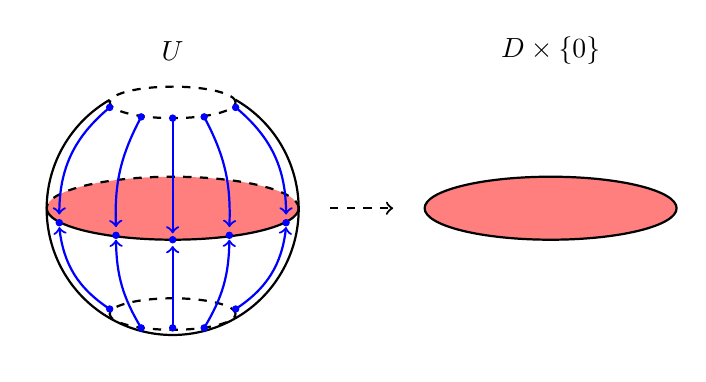
\begin{tikzpicture}[scale=0.8]
                            \shorthandoff{>}

                            \begin{scope}[shift={(-2,0)}]
                                \node at (0,2.5) {$U$};

                                % Color radio medio
                                \fill[red, opacity=0.5] (0,0) ellipse (2 and 0.5);

                                % Radio medio
                                \draw[thick, dashed] (2,0) arc (0:180:2 and 0.5);
                                \draw[thick] (2,0) arc (0:-180:2 and 0.5);

                                % Agujero superior
                                \draw[thick, dashed] (0,1.68) ellipse (1 and 0.25);
                                \draw[thick] (1, 1.72) arc (60:-240:2 and 2);

                                % Puntos superiores
                                \node[draw, circle, fill=blue, blue, inner sep=0.8pt] at (-1,1.6) {};
                                \node[draw, circle, fill=blue, blue, inner sep=0.8pt] at (-0.5,1.45) {};
                                \node[draw, circle, fill=blue, blue, inner sep=0.8pt] at (0,1.43) {};
                                \node[draw, circle, fill=blue, blue, inner sep=0.8pt] at (0.5,1.45) {};
                                \node[draw, circle, fill=blue, blue, inner sep=0.8pt] at (1,1.6) {};

                                % Puntos inferiores
                                \node[draw, circle, fill=blue, blue, inner sep=0.8pt] at (-1.8,-0.23) {};
                                \node[draw, circle, fill=blue, blue, inner sep=0.8pt] at (-0.9,-0.43) {};
                                \node[draw, circle, fill=blue, blue, inner sep=0.8pt] at (0,-0.5) {};
                                \node[draw, circle, fill=blue, blue, inner sep=0.8pt] at (0.9,-0.43) {};
                                \node[draw, circle, fill=blue, blue, inner sep=0.8pt] at (1.8,-0.23) {};
                                
                                % Arcos con flecha
                                \draw[->, bend right=25, blue, thick] (-1,1.6) to (-1.8,-0.1);
                                \draw[->, bend right=15, blue, thick] (-0.5,1.45) to (-0.9,-0.3);
                                \draw[->, blue, thick] (0,1.43) to (0,-0.4);
                                \draw[->, bend left=15, blue, thick] (0.5,1.45) to (0.9,-0.3);
                                \draw[->, bend left=25, blue, thick] (1,1.6) to (1.8,-0.1);

                                % Agujero inferior
                                \draw[thick, dashed] (0,-1.68) ellipse (1 and 0.25);
                                % Puntos inferiores
                                \node[draw, circle, fill=blue, blue, inner sep=0.8pt] at (-1,-1.6) {};
                                \node[draw, circle, fill=blue, blue, inner sep=0.8pt] at (-0.5,-1.9) {};
                                \node[draw, circle, fill=blue, blue, inner sep=0.8pt] at (0,-1.9) {};
                                \node[draw, circle, fill=blue, blue, inner sep=0.8pt] at (0.5,-1.9) {};
                                \node[draw, circle, fill=blue, blue, inner sep=0.8pt] at (1,-1.6) {};
                                % Arcos
                                \draw[->, bend left=25, blue, thick] (-1,-1.6) to (-1.8,-0.3);
                                \draw[->, bend left=15, blue, thick] (-0.5,-1.9) to (-0.9,-0.5);
                                \draw[->, blue, thick] (0,-1.9) to (0,-0.6);
                                \draw[->, bend right=15, blue, thick] (0.5,-1.9) to (0.9,-0.5);
                                \draw[->, bend right=25, blue, thick] (1,-1.6) to (1.8,-0.3);
                            \end{scope}

                            \draw[->, dashed, thick] (0.5,0) -- (1.5,0);

                            \begin{scope}[shift={(4,0)}]
                                \node at (0,2.5) {$\bb{D}\times \{0\}$};

                                % Radio medio
                                \fill[red, opacity=0.5] (0,0) ellipse (2 and 0.5);
                                \draw[thick] (0,0) ellipse (2 and 0.5);
                            \end{scope}
                        \end{tikzpicture}
                    \end{figure}
                    que es simplemente conexo, por lo que:
                    \begin{equation*}
                        \pi_1(U\cap V) = \{1\}
                    \end{equation*}
            \end{itemize}
            En consecuecia, aplicando el Teorema de Seifert-van Kampen, llegamos a que:
            \begin{equation*}
                \pi_1(X) = \{1\}
            \end{equation*}
        \item $X=(\bb{S}^1 \times [-1,1])\cup (\bb{D}\times \{-1,1\})$.

            Tenemos el conjunto:
            \begin{figure}[H]
                \centering
                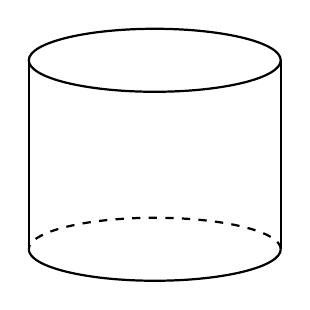
\begin{tikzpicture}[scale=0.8]

                    \draw[thick] (2,2) arc (0:180:2 and 0.5);
                    \draw[thick] (2,2) arc (0:-180:2 and 0.5);
                    \draw[thick, dashed] (2,-1) arc (0:180:2 and 0.5);
                    \draw[thick] (2,-1) arc (0:-180:2 and 0.5);

                    \draw[thick] (2,2) -- (2,-1);
                    \draw[thick] (-2,2) -- (-2,-1);
                \end{tikzpicture}
            \end{figure}
            Si consideramos los conjuntos:
            \begin{equation*}
                U = X\setminus (\bb{D}\times \{1\}), \qquad V = X\setminus(\bb{D}\times \{-1\})
            \end{equation*}
            \begin{figure}[H]
                \centering
                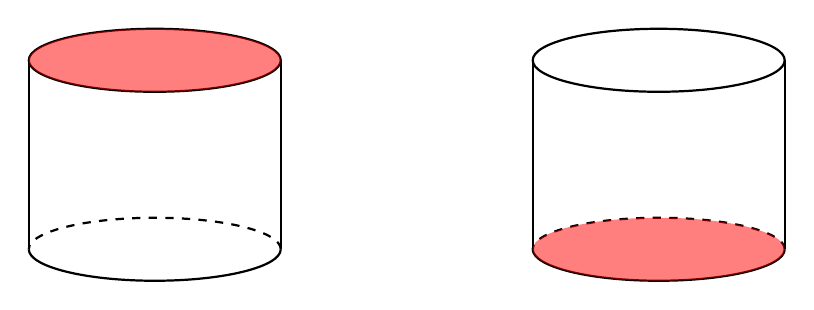
\begin{tikzpicture}[scale=0.8]

                    \draw[thick] (2,2) arc (0:180:2 and 0.5);
                    \draw[thick] (2,2) arc (0:-180:2 and 0.5);
                    \draw[thick, dashed] (2,-1) arc (0:180:2 and 0.5);
                    \draw[thick] (2,-1) arc (0:-180:2 and 0.5);
                    \draw[thick] (2,2) -- (2,-1);
                    \draw[thick] (-2,2) -- (-2,-1);
                    \fill[red, opacity=0.5] (0,2) ellipse (2 and 0.5);

                    \draw[thick] (10,2) arc (0:180:2 and 0.5);
                    \draw[thick] (10,2) arc (0:-180:2 and 0.5);
                    \draw[thick, dashed] (10,-1) arc (0:180:2 and 0.5);
                    \draw[thick] (10,-1) arc (0:-180:2 and 0.5);
                    \draw[thick] (10,2) -- (10,-1);
                    \draw[thick] (6,2) -- (6,-1);
                    \fill[red, opacity=0.5] (8,-1) ellipse (2 and 0.5);
                \end{tikzpicture}
            \end{figure}
            Tenemos que:
            \begin{itemize}
                \item Claramente $X=  U\cup V$.
                \item $U$ y $V$ son abiertos, pues $(\bb{D}\times \{p\})$ es siempre un conjunto cerrado, como producto de cerrados.
                \item $U$, $V$ y $U\cap V$ son claramente\footnote{Habría que justificarlo mejor en un examen.} arcoconexos. 
                \item $U$ tiene a $\bb{D}\times \{-1\}$ como retracto de deformación, por lo que $\pi_1(U) = \{1\}$.
                \item $V$ tiene a $\bb{D}\times \{1\}$ como retracto de deformación, por lo que $\pi_1(V) = \{1\}$.
            \end{itemize}
            Aplicando el Teorema de Seifert-van Kampen, como $\pi_1(U)=\{1\}=\pi_1(V)$, obtenemos que $\pi_1(X) = \{1\}$.
        \item $X = \{(x,y,z)\in \mathbb{R}^3 : x^2+y^2 = {(z+1)}^{2}, -1\leq z\leq 0\}\cup (\bb{S}^2 \cap \{z\geq 0\})$.

            Tratamos de averiguar primero qué conjunto $X$ nos están dando:
            \begin{itemize}
                \item Está claro que la segunda parte de la unión es la ``cáscara'' superior de la esfera de $\mathbb{R}^3$.
                \item Para el primer conjunto de la unión, vemos que a altura $z$ tenemos la circunferencia de centro $0$ y radio $|z+1|$, por lo que podemos pensar en que este conjunto es un cono. Observamos que $|z+1| = 0 \Longleftrightarrow z = -1$, con lo que este primer conjunto es el cono desplazado una unidad hacia los valores negativos de $z$.
            \end{itemize}
            En definitiva, la figura dada es similar a:
            \begin{figure}[H]
                \centering
                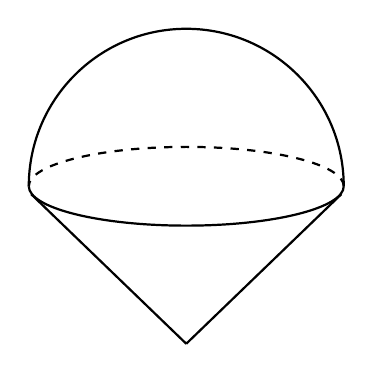
\begin{tikzpicture}
                % Circunferencia
                \draw[thick] (2,0) arc (0:180:2 and 2);
                \draw[thick, dashed] (2,0) arc (0:180:2 and 0.5);
                \draw[thick] (2,0) arc (0:-180:2 and 0.5);
                \draw[thick] (0,-2) -- (-1.97,-0.1);
                \draw[thick] (0,-2) -- (1.97,-0.1);
                \end{tikzpicture}
            \end{figure} 
            Si tomamos ahora:
            \begin{equation*}
                U = X\setminus \{(0,0,1)\}, \qquad V = X\setminus \{(0,0,-1)\}
            \end{equation*}
            Tenemos que:
            \begin{itemize}
                \item Claramente $X=U\cup V$ y $U,V$ son abiertos.
                \item $U$, $V$ y $U\cap V$ son claramente arcoconexos.
                \item $U$ tiene a $(\{0,0,-1\})$ como retracto de deformación, por lo que $U$ es simplemente conexo.
                \item $V$ tiene a $(\{0,0,1\})$ como retracto de deformación, por lo que $V$ es simplemente conexo.
            \end{itemize}
            Aplicando el Teorema de Seifert-van Kampen tenemos que $X$ es simplemente conexo.
        \item $X = S_1 \cup S_2 \cup L$, donde $S_1,S_2$ son cerrados disjuntos simplemente conexos de $\mathbb{R}^n$ y $L\subset \mathbb{R}^n$ es un segmento tal que $L\cap S_i =\{x_i\}$, $i = 1,2$.

            Podemos imaginar que tenemos un conjunto similar a:
            \begin{figure}[H]
                \centering
                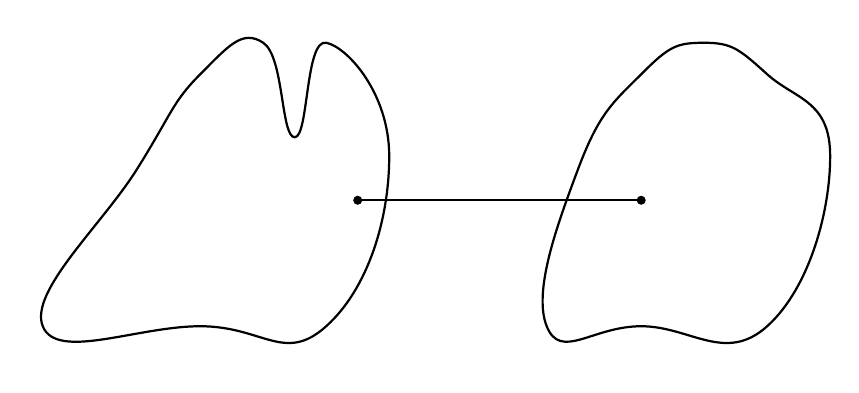
\begin{tikzpicture}[scale=0.8]
                    \shorthandoff{>}
                    \draw[thick] plot[smooth cycle, tension=0.8] coordinates {
                        (-1,0.5) (0,2) (1,2.5) (1.5,1) (2,2.5) (3, 0.7) (2,-2) (0,-2) (-2.5,-2)
                    };
                    \draw[thick] plot[smooth cycle, tension=0.8] coordinates {
                        (6,0.5) (7,2) (8,2.5) (9,2) (10, 0.7) (9,-2) (7,-2) (5.5,-2)
                    };
                    \draw[thick] (2.5,0) -- (7,0);
                    \node[draw, circle, fill=black, inner sep=1pt] at (2.5,0) {};
                    \node[draw, circle, fill=black, inner sep=1pt] at (7,0) {};
                \end{tikzpicture} 
            \end{figure}
            Si consideramos:
            \begin{equation*}
                U = X\setminus S_2, \qquad V = X\setminus S_1
            \end{equation*}
            Tenemos que:
            \begin{itemize}
                \item Claramente $U\cup V = X$.
                \item $U$ y $V$ son abiertos, ya que $S_2$ y $S_1$ son cerrados.
                \item $U$ es arcoconexo, pues $S_1$ y $L$ son arcoconexos (el primero por ser arcoconexo y el segundo por ser imagen por una función continua de un conjunto arcoconexo) que se intersecan en $x_1$. Análogamente, se prueba que $V$ es arcoconexo.
                \item Tenemos que $U\cap V = L\setminus \{x_1,x_2\}$, que claramente es simplemente conexo.
                \item $U$ tiene a $S_1$ como retracto de deformación, por lo que:
                    \begin{equation*}
                        \pi_1(U) = \pi_1(S_1) = \{1\}
                    \end{equation*}
                \item Análogamente $V$ tiene a $S_2$ como retracto de deformación, por lo que:
                    \begin{equation*}
                        \pi_1(V) = \pi_1(S_2) = \{1\}
                    \end{equation*}
            \end{itemize}
            Aplicando el Teorema de Seifert-van Kampen obtenemos que $\pi_1(X) = \{1\}$.
        \item $X\subset \mathbb{R}^3$ es la unión de una circunferencia y de una esfera que se tocan en un único punto.

            Si consideramos $X = S\cup C$ con $S$ una esfera de $\mathbb{R}^3$, $C$ una circunferencia de $\mathbb{R}^3$ y $S\cap C = \{x_0\}$:
            \begin{figure}[H]
                \centering
                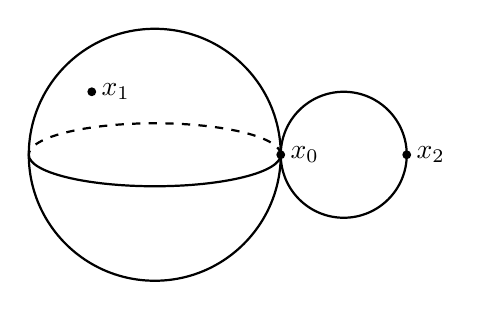
\begin{tikzpicture}[scale=0.8]
                    \shorthandoff{>}
                    % Esfera
                    \draw[thick] (0,0) circle [radius=2];
                    \draw[thick, dashed] (2,0) arc (0:180:2 and 0.5);
                    \draw[thick] (2,0) arc (0:-180:2 and 0.5);
                    \draw[thick] (3,0) circle [radius=1];

                    \fill (-1,1) circle(2pt) node[right] {$x_1$};
                    \fill (2,0) circle(2pt) node[right] {$x_0$};
                    \fill (4,0) circle(2pt) node[right] {$x_2$};
                \end{tikzpicture} 
            \end{figure}
            Si consideramos:
            \begin{gather*}
                U = X\setminus \{x_1\}, \quad x_1\in S\setminus \{x_0\} \\
                V= X\setminus\{x_2\}, \quad x_2\in C\setminus\{x_0\}
            \end{gather*}
            Tenemos que:
            \begin{itemize}
                \item Claramente $X=U\cup V$ y $U,V$ son abiertos.
                \item $U$ es arcoconexo, como unión de $S\setminus \{x_1\}$, que es homeomorfo a $\mathbb{R}^2$ luego es arcoconexo, y de $C$. Notemos que $(S\setminus \{x_1\})\cap C = \{x_0\}$.
                \item $V$ es arcoconexo, como unión de $S$, que es arcoconexo con cada uno de los arcos que unen $x_0$ con $x_2$ (abiertos en $x_2$), cada uno de ellos es arcoconexo e intersecan a $S$ en $x_0$.
                \item $U\cap V$ es arcoconexo, como unión de $S\setminus \{x_1\}$ con cada uno de los arcos, ya que todos ellos se intersecan en $\{x_0\}$.
                \item $U$ tiene a $C$ como retracto de deformación, por lo que:
                    \begin{equation*}
                        \pi_1(U) = \pi_1(C) \cong \pi_1(\bb{S}^1) \cong \mathbb{Z}
                    \end{equation*}
                \item $V$ tiene a $S$ como retracto de deformación, por lo que:
                    \begin{equation*}
                        \pi_1(V) = \pi_1(S) \cong \pi_1(\bb{S}^2) = \{1\}
                    \end{equation*}
                \item $U\cap V$ tiene a $\{x_0\}$ como retracto de deformación, por lo que es simplemente conexo.
            \end{itemize}
            Aplicando el Teorema de Seifert-van Kampen obtenemos que:
            \begin{equation*}
                \pi_1(X) = \pi_1(U) \ast \pi_1(V) \cong \mathbb{Z}\ast \{1\} = \mathbb{Z}
            \end{equation*}
        \item $X = \bb{S}^2\cup \{(x,y,z)\in \mathbb{R}^3 : y^2 + {(z-2)}^{2} = 1\}\cup \{(x,y,z)\in \mathbb{R}^3 : y^2 + {(z+2)}^{2}=1\}$.
            $X$ está compuesto por la unión de la esfera de $\mathbb{R}^3$ junto con dos cilindros de radio 1 a lo largo del eje $x$ (tienen altura infinita), de forma que cada cilindor tiene un único punto de intersección con la esfera.
            \begin{figure}[H]
                \centering
                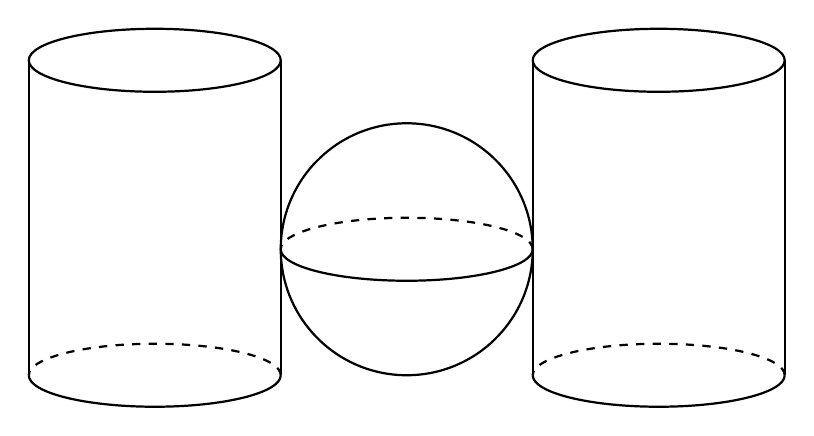
\begin{tikzpicture}[scale=0.8]

                    \draw[thick] (2,4) arc (0:180:2 and 0.5);
                    \draw[thick] (2,4) arc (0:-180:2 and 0.5);
                    \draw[thick, dashed] (2,-1) arc (0:180:2 and 0.5);
                    \draw[thick] (2,-1) arc (0:-180:2 and 0.5);
                    \draw[thick] (2,4) -- (2,-1);
                    \draw[thick] (-2,4) -- (-2,-1);

                    \draw[thick] (10,4) arc (0:180:2 and 0.5);
                    \draw[thick] (10,4) arc (0:-180:2 and 0.5);
                    \draw[thick, dashed] (10,-1) arc (0:180:2 and 0.5);
                    \draw[thick] (10,-1) arc (0:-180:2 and 0.5);
                    \draw[thick] (10,4) -- (10,-1);
                    \draw[thick] (6,4) -- (6,-1);

                    \draw[thick] (4,1) circle [radius=2];
                    \draw[thick, dashed] (6,1) arc (0:180:2 and 0.5);
                    \draw[thick] (6,1) arc (0:-180:2 and 0.5);
                \end{tikzpicture}
            \end{figure}
            En primer lugar, observamos que un retracto de deformación de $X$ es el conjunto $Y$:
            \begin{equation*}
                Y = \{(0,y,z)\in \mathbb{R}^3 : y^2+{(z-2)}^{2}=1 \} \cup \{(0,y,z)\in \mathbb{R}^3 : y^2 + {(z+1)}^{2}=1\} \cup \bb{S}^2
            \end{equation*}
            \begin{figure}[H]
                \centering
                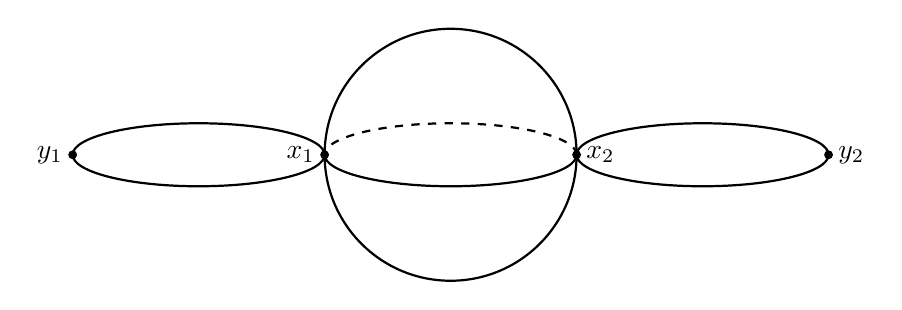
\begin{tikzpicture}[scale=0.8]
                    \draw[thick] (10,1) arc (0:180:2 and 0.5);
                    \draw[thick] (10,1) arc (0:-180:2 and 0.5);

                    \draw[thick] (2,1) arc (0:180:2 and 0.5);
                    \draw[thick] (2,1) arc (0:-180:2 and 0.5);

                    \draw[thick] (4,1) circle [radius=2];
                    \draw[thick, dashed] (6,1) arc (0:180:2 and 0.5);
                    \draw[thick] (6,1) arc (0:-180:2 and 0.5);

                    \fill (2,1) circle(2pt) node[left] {$x_1$};
                    \fill (6,1) circle(2pt) node[right] {$x_2$};
                    \fill (-2,1) circle(2pt) node[left] {$y_1$};
                    \fill (10,1) circle(2pt) node[right] {$y_2$};
                \end{tikzpicture}
            \end{figure}
            Si nombramos a cada una circunferencia $C_1$ y a la otra $C_2$ tendremos entonces que:
            \begin{equation*}
                Y = C_1\cup C_2 \cup \bb{S}^2, \qquad C_1\cap \mathbb{S}^2 = \{x_1\}, \qquad C_2\cap \mathbb{S}^2 = \{x_2\}
            \end{equation*}
            En este punto, consideramos los conjuntos:
            \begin{gather*}
                U = X\setminus \{y_2\}, \quad y_2\in C_2\setminus\{x_2\} \\
                V = X\setminus \{y_1\}, \quad y_1\in C_1\setminus\{x_1\} \\
            \end{gather*}
            De esta forma:
            \begin{itemize}
                \item Tenemos claramente que $U$ y $V$ son abiertos con $X=U\cup V$.
                \item $U$, $V$ y $U\cap V$ son arcoconexos, todos ellos por ser unión de conjuntos arcoconexos que se intersecan en un punto.
                \item $U$ tiene a $C_1\cup\mathbb{S}^2$ como retracto de deformación, y en el apartado anterior vimos que dicho espacio topológico tiene grupo fundamental $\mathbb{Z}$, por lo que $\pi_1(U)\cong \mathbb{Z}$.
                \item Análogamente, $V$ tiene a $C_2\cup\mathbb{S}^2$ como retracto de deformación, por lo que $\pi_1(V)\cong \mathbb{Z}$.
                \item $U\cap V$ tiene a $\mathbb{S}^2$ como retracto de deformación, por lo que $U\cap V$ es simplemente conexo.
            \end{itemize}
            En definitiva, aplicando el Teorema de Seifert-van Kampen, obtenemos que:
            \begin{equation*}
                \pi_1(X) = \pi_1(Y) \cong \mathbb{Z}\ast \mathbb{Z}
            \end{equation*}
        \item $X = S_1 \cup (\bb{S}^1 \times \{0\})\cup S_2$, donde $S_1$ y $S_2$ son, respectivamente, las esferas de radio 1 centradas en el $(0,-2,0)$ y en el $(0,2,0)$.
            Tenemos el conjunto:
            \begin{figure}[H]
                \centering
                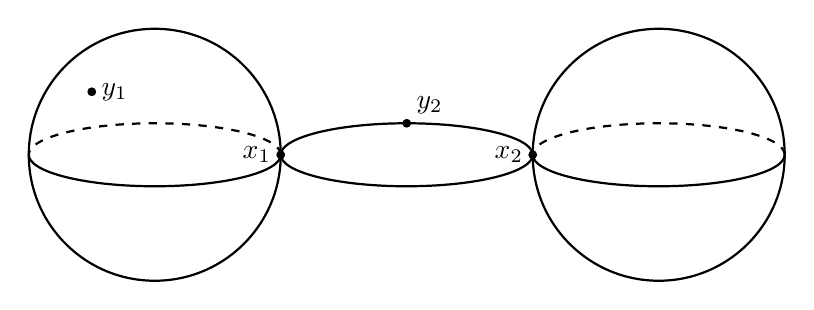
\begin{tikzpicture}[scale=0.8]
                    \draw[thick] (8,1) arc (0:180:2 and 0.5);
                    \draw[thick] (8,1) arc (0:-180:2 and 0.5);

                    \draw[thick] (2,1) circle [radius=2];
                    \draw[thick, dashed] (4,1) arc (0:180:2 and 0.5);
                    \draw[thick] (4,1) arc (0:-180:2 and 0.5);

                    \draw[thick] (10,1) circle [radius=2];
                    \draw[thick, dashed] (12,1) arc (0:180:2 and 0.5);
                    \draw[thick] (12,1) arc (0:-180:2 and 0.5);

                    \fill (4,1) circle(2pt) node[left] {$x_1$};
                    \fill (1,2) circle(2pt) node[right] {$y_1$};
                    \fill (8,1) circle(2pt) node[left] {$x_2$};
                    \fill (6,1.5) circle(2pt) node[above right] {$y_2$};
                \end{tikzpicture}
            \end{figure}
            Notando $S_i\cap (\mathbb{S}^1\times \{0\}) = \{x_i\}$ para $i \in \{1,2\}$, definiendo los conjuntos:
            \begin{gather*}
                U = X\setminus \{y_1\}, \quad y_1 \in S_1\setminus \{x_1\} \\
                V = X\setminus \{y_2\}, \quad y_2 \in (\mathbb{S}^1\times \{0\})\setminus \{x_1,x_2\}
            \end{gather*}
            Tenemos que:
            \begin{itemize}
                \item $U$ y $V$ son abiertos, con $X=U\cup V$.
                \item Claramente $U$, $V$ y $U\cap V$ son arcoconexos.
                \item $U$ tiene a $S_2\cup (\mathbb{S}^1\times \{0\})$ como retracto de deformación, y en el apartado $f)$ vimos que este espacio topológico tiene un grupo fundamental isomorfo a $\mathbb{Z}$, por lo que $\pi_1(U)\cong \mathbb{Z}$.
                \item $V$ tiene a:
                    \begin{equation*}
                        S_1\cup S_2 \cup ((\mathbb{S}^1\cap \{(x,y)\in \mathbb{R}^2 : x\leq 0\})\times \{0\})
                    \end{equation*}
                    como retracto de deformación:
                    \begin{figure}[H]
                        \centering
                    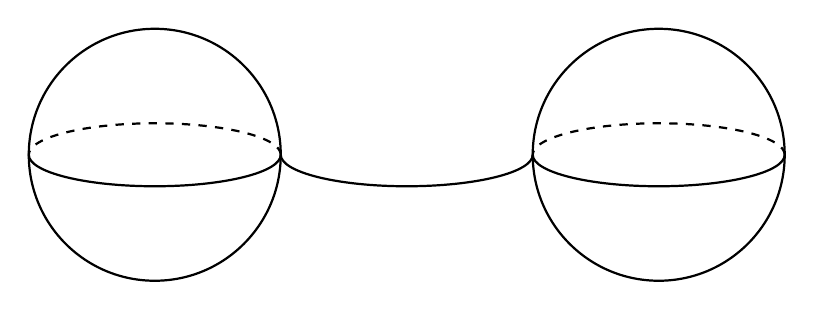
\begin{tikzpicture}[scale=0.8]
                        \draw[thick] (8,1) arc (0:-180:2 and 0.5);

                        \draw[thick] (2,1) circle [radius=2];
                        \draw[thick, dashed] (4,1) arc (0:180:2 and 0.5);
                        \draw[thick] (4,1) arc (0:-180:2 and 0.5);

                        \draw[thick] (10,1) circle [radius=2];
                        \draw[thick, dashed] (12,1) arc (0:180:2 and 0.5);
                        \draw[thick] (12,1) arc (0:-180:2 and 0.5);
                    \end{tikzpicture}
                    \end{figure}
                    Por lo que $\pi_1(V) = \{1\}$, tal y como se vio en el apartado $d)$.
                \item $U\cap V$ tiene a $S_2$ como retracto de deformación, por lo que $U\cap V$ es simplemente conexo.
            \end{itemize}
            Aplicando el Teorema de Seifert-van Kampen obtenemos que:
            \begin{equation*}
                \pi_1(X) \cong \mathbb{Z}\ast \{1\} = \mathbb{Z}
            \end{equation*}
        \item $X\subset \mathbb{R}^2$ es la unión de las tres circunferencias de radio 1 centradas en los puntos $(-2,0)$, $(0,0)$ y $(2,0)$.

            Tenemos que $X= S_{-2}\cup S_0\cup S_2$, con $S_{-2}\cap S_0 = \{x_1\}$ y $S_0\cap S_2 = \{x_2\}$:
            \begin{figure}[H]
                \centering
            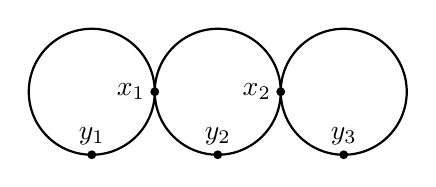
\begin{tikzpicture}[scale=0.8]
                \draw[thick] (2,1) circle [radius=1];
                \draw[thick] (4,1) circle [radius=1];
                \draw[thick] (6,1) circle [radius=1];
                \fill (3,1) circle(2pt) node[left] {$x_1$};
                \fill (5,1) circle(2pt) node[left] {$x_2$};
                \fill (2,0) circle(2pt) node[above] {$y_1$};
                \fill (4,0) circle(2pt) node[above] {$y_2$};
                \fill (6,0) circle(2pt) node[above] {$y_3$};
            \end{tikzpicture}
            \end{figure}
            Si consideramos $y_1\in S_{-2}\setminus \{x_1\}$, $y_2\in S_0\setminus\{x_1,x_2\}$, $y_3\in S_2\setminus \{x_2\}$, podemos definir los conjuntos:
            \begin{equation*}
                U = X\setminus \{y_1,y_2\}, \qquad V = X\setminus \{y_3\}
            \end{equation*}
            Y tenemos que:
            \begin{itemize}
                \item Claramente $U$ y $V$ son abiertos con $X=U\cup V$.
                \item Claramente $U$, $V$ y $U\cap V$ son arcoconexos.
                \item $U$ tiene a $S_2$ como retracto de deformación, por lo que $\pi_1(U)\cong \mathbb{Z}$.
                \item $V$ tiene a $Y = S_{-2}\cup S_0$ como retracto de deformación, y tomando:
                    \begin{equation*}
                        W = Y\setminus \{y_1\}, \qquad Z = Y\setminus \{y_2\}
                    \end{equation*}
                    tenemos que:
                    \begin{itemize}
                        \item $Y=W\cup Z$ con $W$ y $Z$ abiertos arcoconexos, con $W\cap Z$ arcoconexo.
                        \item $W$ tiene a $S_2$ como retracto de deformación, por lo que $\pi_1(W)\cong \mathbb{Z}$.
                        \item $Z$ tiene a $S_0$ como retracto de deformación, por lo que $\pi_1(Z)\cong \mathbb{Z}$.
                        \item $W\cap Z$ tiene a $x_1$ como retracto de deformación, por lo que $W\cap Z$ es simplemente conexo.
                    \end{itemize}
                    De aquí deducimos aplicando el Teorema de Seifert-van Kampen que $\pi_1(V) = \pi_1(Y) \cong \mathbb{Z}\ast\mathbb{Z}$.
                \item $U\cap V$ tiene a $\{x_2\}$ como retracto de deformación, por lo que $U\cap V$ es simplemente conexo.
            \end{itemize}
            En definitiva, por el Teorema de Seifert-van Kampen deducimos que:
            \begin{equation*}
                \pi_1(X) \cong (\mathbb{Z}\ast\mathbb{Z})\ast\mathbb{Z} = \mathbb{Z}\ast\mathbb{Z}\ast\mathbb{Z}
            \end{equation*}
            Observemos que un razonamiento similar puede hacerse para el caso de $n$ circunferencias de forma que la intersección dos a dos de ellas es unitaria, obteniendo que la unión de dichas $n$ circunferencias sería $\ast_{i=1}^n \mathbb{Z}$.
        \item $X = \bb{S}^1\cup [(-1,0), (1,0)]$.

            Tenemos el conjunto:
            \begin{figure}[H]
                \centering
            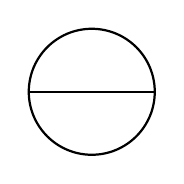
\begin{tikzpicture}[scale=0.8]
                \draw[thick] (0,1) circle [radius=1];
                \draw[thick] (-1,1) -- (1,1);
            \end{tikzpicture}
            \end{figure}
            Si consideramos:
            \begin{equation*}
                U = X\setminus \{(0,0)\}, \qquad V = X\setminus \{(0,1)\}
            \end{equation*}
            tenemos que:
            \begin{itemize}
                \item $X=U\cup V$ con $U$ y $V$ abiertos.
                \item $U$, $V$ y $U\cap V$ son arcoconexos.
                \item $U$ tiene a $\mathbb{S}^1$ como retracto de deformación, por lo que $\pi_1(U)\cong \mathbb{Z}$.
                \item $V$ tiene a:
                    \begin{equation*}
                        (\{(x,y):y\leq 0\}\cap \mathbb{S}^1)\cup [(-1,0),(1,0)]
                    \end{equation*}
                    como retracto de deformación, y este último es homeomorfo a $\mathbb{S}^1$, por lo que $\pi_1(V)\cong \mathbb{Z}$.
                \item $U\cap V$ es contráctil, ya que tiene por ejemplo a $\{(0,-1)\}$ como retracto de deformación, por lo que $U\cap V$ es simplemente conexo.
            \end{itemize}
            En definitiva, aplicando el Teorema de Seifert-van Kampen tenemos que:
            \begin{equation*}
                \pi_1(X) = \mathbb{Z}\ast\mathbb{Z}
            \end{equation*}
    \end{enumerate}
\end{ejercicio}

\begin{ejercicio}
    Razona si son verdaderas o falsas las siguientes afirmaciones:
    \begin{enumerate}[label=\alph*)]
        \item Sean $\alpha_1,\alpha_2,\beta_1,\beta_2\in \Omega(X,x_0)$  con $[\alpha_1\ast \beta_1] = [\alpha_2\ast \beta_2]$. Entonces $[\alpha_1] = [\alpha_2]$ y $[\beta_1] = [\beta_2]$.\\

            Es falsa, puesto que si consideramos $X=\bb{S}^1$, $x_0 =(1,0)$, el arco:
            \begin{equation*}
                \alpha(t) = (\cos(2\pi t), \sen(2\pi t)) \qquad \forall t\in [0,1]
            \end{equation*}
            Y tomamos:
            \begin{equation*}
                \alpha_1 = \alpha = \beta_2, \qquad \alpha_2 = \varepsilon_{x_0} = \beta_1
            \end{equation*}
            Tenemos que $[\alpha_1] \neq [\alpha_2]$, $[\beta_1]\neq[\beta_2]$ y $[\alpha_1\ast \beta_1] = [\alpha_2\ast \beta_2]$.
        \item Sean $f:A\to Y$ una aplicación continua con $A\subset X$ y $X$ simplemente conexo. Si existe $F:X\to Y$ continua con $F\big|_A = f$, entonces $f_\ast$ es trivial.\\

            Es verdadera, como $F$ es una extensión de $f$, tenemos que $f\circ i = F$, es decir:
            \begin{figure}[H]
                \centering
                \shorthandoff{""}
                \begin{tikzcd}
                    {A} \arrow[r, "i", hook] \arrow[rr, "f", bend right=49] & {X} \arrow[r, "F"] & {Y}
                \end{tikzcd}
                \shorthandon{""}
            \end{figure}
            \noindent
            Y como cada una de ellas es continua, podemos inducir el diagrama a grupos fundamentales, obteniendo para cada $x_0\in A$:
            \begin{figure}[H]
                \centering
                \shorthandoff{""}
                \begin{tikzcd}
                    {\pi_1(A,x_0)} \arrow[r, "i_\ast", hook] \arrow[rr, "f_\ast", bend right] & {\pi_1(X,x_0)} \arrow[r, "F_\ast"] & {\pi_1(Y,f(x_0))}
                \end{tikzcd}
                \shorthandon{""}
            \end{figure}
            de donde:
            \begin{equation*}
                f_\ast([\alpha]_A) = F_\ast(i_\ast([\alpha]_{A})) = F_\ast({[\alpha]}_{X}) \AstIg F_\ast([\varepsilon_{x_0}]_{X}) = [\varepsilon_{f(x_0)}]_Y \qquad \forall [\alpha]_A \in \pi_1(A,x_0)
            \end{equation*}
            donde en $(\ast)$ hemos usado que $X$ es simplemente conexo.
        \item Si $f:X\to Y$ es continua y nulhomótopa, entonces $f_\ast$ es trivial.

            Veradera, si $f:X\to Y$ es continua y nulhomótopa, existe entonces una constante $y_0\in Y$ de forma que la aplicación constantemente igual a $y_0$
            \Func{c}{X}{Y}{x}{y_0}
            sea homotópica a $f$, es decir, existe una aplicación continua $H:X\times [0,1]\to Y$ de forma que:
            \begin{equation*}
                H(x,0) = f(x), \qquad H(x,1) = c(x) = y_0 \qquad \forall x\in X
            \end{equation*}
            En este caso, hemos visto en teoría que para cada $x_0\in X$ existe un isomorfismo $\varphi:\pi_1(Y,f(x_0))\to\pi_1(Y,y_0)$ que hace conmutar el siguiente diagrama:
            \begin{figure}[H]
                \centering
                \shorthandoff{""}
                \begin{tikzcd}
                                                                               &  & {\pi_1(Y,f(x_0))} \arrow[dd, "\varphi"] \\
                    {\pi_1(X,x_0)} \arrow[rru, "f_\ast"] \arrow[rrd, "c_\ast"] &  &                                         \\
                                                                               &  & {\pi_1(Y,y_0)}                         
                \end{tikzcd}
                \shorthandon{""}
            \end{figure}
            \noindent
            De donde deducimos que:
            \begin{equation*}
                f_\ast = \varphi^{-1}\circ c_\ast
            \end{equation*}
            Luego si tomamos $\alpha\in \Omega(X,x_0)$, tenemos que:
            \begin{equation*}
                f_\ast([\alpha]) = \varphi^{-1}(c_\ast([\alpha])) = \varphi^{-1}([c \circ \alpha]) = \varphi^{-1}([\varepsilon_{y_0}]) = [\varepsilon_{f(x_0)}]
            \end{equation*}
            de donde deducimos que $f_\ast$ es trivial.
        \item Si $f:X\to \bb{S}^n$ es continua y no sobreyectiva, entonces es nulhomótopa.

            Verdadera, si $f$ no es sobreyectiva existirá entonces $x_0\in \bb{S}^n$ de forma que $x_0\notin f(X)$. Si pensamos ahora en unir cada punto $f(x)$ con $-x_0$ podemos hacerlo a lo largo de $\bb{S}^n$:
            \begin{figure}[H]
                \centering
                \begin{tikzpicture}[scale=0.8]
                    \shorthandoff{>}
                    % Esfera
                    \draw[thick] (0,0) circle [radius=2];
                    \draw[thick, dashed] (2,0) arc (0:180:2 and 0.5);
                    \draw[thick] (2,0) arc (0:-180:2 and 0.5);

                    % Puntos alpha
                    \node[draw, circle, fill=black, inner sep=1pt, label=left:$-x_0$] at (1,1) {};
                    \node[draw, circle, fill=black, inner sep=1pt, label=left:$x_0$] at (-0.8,-0.8) {};
                    \node[draw, circle, fill=black, inner sep=1pt, label=left:$f(x)$] at (1,-1) {};

                    % beta
                    \draw[thick, violet, bend right=15, -Stealth] (1,-1) to (1,1);
                \end{tikzpicture} 
            \end{figure}
            \noindent
            De esta forma, definimos $H:X\times [0,1]\to \bb{S}^n$ dada por:
            \begin{equation*}
                H(x,t) = \dfrac{(1-t)f(x) + t(-x_0)}{|(1-t)f(x) + t(-x_0)|}
            \end{equation*}
            Observamos que:
            \begin{equation*}
                |(1-t)f(x) + t(-x_0)| = 0 \Longleftrightarrow (1-t)f(x) = tx_0 \qquad \forall t\in [0,1]
            \end{equation*}
            Como $f(x),x_0\in \bb{S}^n$, esto último solo puede suceder si:
            \begin{itemize}
                \item $f(x) = x_0$, pero $x_0\notin f(X)$.
                \item $f(x) = -x_0$, pero en este caso tenemos $(1-t)f(x) + t(-x_0) = 1$.
            \end{itemize}
            Por lo que el denominador nunca se anula, lo que nos permite obtener la función $H$ continua, que hemos definido, que verifica:
            \begin{equation*}
                H(x,0) = f(x), \qquad H(x,1) = -x_0 \qquad \forall x\in X
            \end{equation*}
            Por lo que $f$ es homotópica a la función $X\to \bb{S}^n$ constantemente igual a $-x_0$, de donde $f$ es nulhomótopa.
        \item Si $X$ es simplemente conexo y $A\subset X$ un retracto de $X$, entonces $A$ es simplemente conexo. 

            Verdadera, puesto que si $A$ es un retracto de $X$, entonces fijado $x_0\in A$ la aplicación inclusión $i:A\to X$ induce un monomorfismo entre grupos fundamentales $i_\ast:\pi_1(A,x_0)\to \pi_1(X,x_0)$. Como
            \begin{equation*}
                \pi_1(X,x_0) \cong \{1\}
            \end{equation*}
            ha de ser $\pi_1(X,x_0)\cong \{1\}$. Además, por ser $A$ un retracto de $X$, existe una aplicación $r:X\to A$ continua de forma que $r(a) = a \quad \forall a\in A$, por lo que $A = r(X)$, y como $X$ es arcoconexo $A$ también debe serlo.
        \item Si $f:X\to Y$ es continua e inyectiva con $f(x_0)=y_0$ entonces el homomorfismo $f_\ast:\pi_1(X,x_0)\to \pi_1(Y,y_0)$ es un monomorfismo.

            Falsa, puesto que la aplicación inclusión
            \Func{i}{\bb{S}^1}{\bb{R}^2}{x}{x}
            es continua e inyectiva, y si tomamos $x_0\in X$, $y_0 = f(x_0)$, tenemos el homomorfismo $i_\ast:\pi_1(\bb{S}^1,x_0)\to \pi_1(\mathbb{R}^2, x_0)$ que no es inyectivo, puesto que:
            \begin{equation*}
                \pi_1(\bb{S}^1,x_0) \cong \mathbb{Z}, \qquad \pi_1(\mathbb{R}^2,x_0)\cong \{1\}
            \end{equation*}
        \item Sea $f:X\to Y$ una equivalencia homotópica y $A\subset X$. La restricción $f\big|_A:A\to f(A)$ es una equivalencia homotópica. % // TODO: REVISAR
            
            Falsa: sean $X=\mathbb{R}^2\setminus \{(0,0)\}$ y $Y = \bb{S}^1$, sabemos que $Y$ es retracto de deformación de $X$, por lo que existe una aplicación continua $r:X\to Y$ dada por:
            \begin{equation*}
                r(x) = \frac{x}{|x|}
            \end{equation*}
            de forma que su composición con la inclusión $Y\stackrel{i}{\hookrightarrow} X$ es homotópica a la identidad. Tomando por tanto $f=r$ y $g=i$ tenemos que $r$ es una equivalencia homotópica.
            \begin{description}
                \item [Opción 1.] 
                    Si consideramos el conjunto: 
                    \begin{equation*}
                        A = \left\{(r(\theta)\cos\theta, r(\theta)\sen\theta) : r(\theta) = 1 + \frac{\theta}{2\pi}, \theta \in [0,2\pi]\right\}
                    \end{equation*}

                    \begin{figure}[H]
                        \centering
                    \begin{tikzpicture}

                        % Ejes coordenados
                        \draw[-Stealth] (-1.4,0) -- (2.2,0);
                        \draw[-Stealth] (0,-1.4) -- (0,1.4);

                        % Punto (0,0) quitado: círculo no relleno
                        \draw[fill=white,thick] (0,0) circle (0.05);

                        % Circunferencia de radio 1
                        \draw[thick] (0,0) circle (1);

                        % Espiral: r = 1 + theta/(2*pi), theta in [0, 2*pi]
                        \draw[red, thick, domain=0:360, samples=200]
                            plot ({(1 + \x/360)*cos(\x)}, {(1 + \x/360)*sin(\x)});
                        \fill (1,1) node[right] {$A$};
                    \end{tikzpicture}
                    \caption{Representación gráfica de $X$, $Y$ y $A$.}
                    \end{figure}
                    \noindent
                    Tenemos la aplicación $r\big|_A:A\to \bb{S}^1$, que no puede ser una equivalencia homotópica, ya que $A$ es simplemente conexo y $\bb{S}^1$ tiene un grupo isomorfo a $\mathbb{Z}$ como grupo fundamental.
                \item [Opción 2.] Si consideramos el conjunto:
                    \begin{equation*}
                        A = B((1.5,1.5), 0.5)
                    \end{equation*}
                    \begin{figure}[H]
                        \centering
                    \begin{tikzpicture}

                        % Ejes coordenados
                        \draw[-Stealth] (-1.4,0) -- (2.2,0);
                        \draw[-Stealth] (0,-1.4) -- (0,1.4);

                        % Punto (0,0) quitado: círculo no relleno
                        \draw[fill=white,thick] (0,0) circle (0.05);

                        % Circunferencia de radio 1
                        \draw[thick] (0,0) circle (1);
                        % Circunferencia pequeña
                        \draw[red, thick] (1.5,1.5) circle (0.5);

                        \draw[dashed] (0,0) -- (1.1,1.8);
                        \draw[dashed] (0,0) -- (1.8,1.1);

                        \fill (1.2,1.5) node[right] {$A$};
                        \fill[blue] (0.9,0.4) node[right] {$r(A)$};

                        \draw[blue, thick] (0.5,0.87) arc[start angle=60, end angle=30, radius=1];
                    \end{tikzpicture}
                    \caption{Representación gráfica de $X$, $Y$, $A$ y $r(A)$ en azúl.}
                    \end{figure}
                    \noindent
                    Tenemos la aplicación $r\big|_A:A\to r(A)$, que no puede ser una equivalencia homotópica, ya que $A$ es homeomorfo a $\bb{S}^1$, por lo que tiene grupo fundalmental isomorfo a $\mathbb{Z}$ y $r(A)$ es un subconjunto simplemente conexo de $\bb{S}^1$.
            \end{description}
        \item $\bb{S}^1$ no tiene ningún retracto de deformación $D\neq \bb{S}^1$.

            Verdadera: por reducción al absurdo, si fuese $D\subsetneq \bb{S}^1$ un retracto de deformación suyo, como $D\neq \bb{S}^1$ ha de existir $x_0\in \bb{S}^1$ de forma que $D\subseteq \bb{S}^1\setminus \{x_0\}$. Como $\bb{S}^1\setminus \{x_0\}$ es homeomorfo a $\mathbb{R}$, $D$ es homeomorfo a un subconjunto de $\mathbb{R}$, y como $D$ es un retracto de deformación de $\bb{S}^1$ ha de existir una función $r:\bb{S}^1\to D$ continua de forma que $D = r(\bb{S}^1)$. Como $\bb{S}^1$ es conexo, $D$ ha de ser homeomorfo a un subconjunto conexo de $\mathbb{R}$, es decir, a un intervalo, que siempre es simplemente conexo, por lo que $D$ es simplemente conexo, pero por ser retracto de deformación de $\bb{S}^1$ debería tener grupo fundamental isomorfo a $\mathbb{Z}$, hemos llegado a una \underline{contradicción}.
        \item Existe un homeomorfismo de $\mathbb{R}^2$ que intercambia las componentes conexas de $\mathbb{R}^2\setminus \bb{S}^1$.

            Falsa: por reducción al absurdo, si existiera $f:\mathbb{R}^2\to \mathbb{R}^2$ que intercambia las componentes conexas de $\mathbb{R}^2\setminus \bb{S}^1$, es decir, que si:
            \begin{equation*}
                A = \{x\in \mathbb{R}^2 : |x| > 1\}, \qquad B = \{x\in \mathbb{R}^2 : |x|<1\}
            \end{equation*}
            se tiene $f(A) = B$, $f(B) = A$; tendríamos entonces al considerar $f\big|_A$ que $A$ es homeomorfo a $B$, por lo que ambos han de tener el mismo grupo fundamental. Sin embargo:
            \begin{itemize}
                \item $B$ es estrellado, por lo que tiene grupo fundamental trivial.
                \item $A$ tiene como retracto de deformación el conjunto:
                    \begin{equation*}
                        S = \{x\in \mathbb{R}^2 : |x| = 2\}
                    \end{equation*}
                    que es una homotecia de $\bb{S}^1$, luego $S\cong\bb{S}^1$, de donde deducimos que:
                    \begin{equation*}
                        \pi_1(A) = \pi_1(S) = \pi_1(\bb{S}^1)\cong \mathbb{Z}
                    \end{equation*}
            \end{itemize}
            Vemos que $\pi_1(A)\neq \pi_1(B)$, contradicción que viene de suponer la existencia del homeomorfismo $f$ que intercambia $A$ y $B$.
        \item Si $A$ es un retracto del disco unidad cerrado de $\mathbb{R}^2$, entonces toda aplicación continua $f:A\to A$ tiene al menos un punto fijo.

            Verdadera, si $A$ es un retracto de $\bb{D}$ tenemos entonces que existe $r:\bb{D}\to A$ continua de forma que $r(a) = a\quad \forall a\in A$. Sea ahora una aplicación continua $f:A\to A$, tenemos que la aplicación $h:\bb{D}\to \bb{D}$ dada como la siguiente composición de funciones continuas:
            \begin{figure}[H]
                \centering
                \shorthandoff{""}
                \begin{tikzcd}
                    \mathbb{D} \arrow[r, "r"] & A \arrow[r, "f"] & A \arrow[r, "i", hook] & \mathbb{D}
                \end{tikzcd}
                \shorthandon{""}
            \end{figure}
            tiene un punto fijo por el Teorema de Brouwer, es decir, existe $x_0\in \bb{D}$ de forma que:
            \begin{equation*}
                x_0 = h(x_0) = i(f(r(x_0))) = f(r(x_0))
            \end{equation*}
            como $f$ toma valores en $A$ tenemos que $x_0\in A$, por lo que $r(x_0 ) =x_0$, con lo que:
            \begin{equation*}
                x_0 = f(r(x_0)) = f(x_0)
            \end{equation*}
            Por lo que $f$ tiene un punto fijo.
    \end{enumerate}
\end{ejercicio}
